
\chapter{Coordination Avoidance and RAMP Transactions}
\label{c.ramp}

In the previous chapter, we identified several existing isolation and
distributed consistency guarantees as coordination-free. Our goal was
proof-of-concept algorithms and systems support for these levels. In
this section, we go further. First, we develop a \textit{new} isolation
model that is tailored to a set of existing use cases for which there
is no existing, sufficiently powerful \iconfluent semantics. Second,
we develop high performance algorithms for enforcing those
semantics. 

Specifically, in this chapter, we address a largely underserved class
of applications requiring multi-partition, atomically
visible\footnote{\label{atomicnote}Our use of ``atomic''
  (specifically, Read Atomic isolation) concerns all-or-nothing
  \textit{visibility} of updates (i.e., the ACID isolation effects of
  ACID atomicity; Section~\ref{sec:ra-def}). This differs from uses of
  ``atomicity'' to denote serializability~\cite{bernstein-book} or
  linearizability~\cite{dcomp-book}.}  \textit{transactional} access:
cases where all or none of each transaction's effects should be
visible. In fact, this access corresponds to two semantics from the
previous chapter: MAV combined with Cut Isolation. The status quo for
these multi-partition atomic transactions provides an uncomfortable
choice between algorithms that are fast but deliver inconsistent
results and algorithms that deliver consistent results but are often
slow and unavailable under failure. Many of the largest modern,
real-world systems opt for protocols that guarantee fast and scalable
operation but provide few---if any---transactional semantics for
operations on arbitrary sets of data
items~\cite{tao,bigtable,pnuts,dynamo,2pc-scalability,espresso,rainbird}. This
may lead to anomalous behavior for several use cases requiring atomic
visibility, including secondary indexing, foreign key constraint
enforcement, and materialized view maintenance
(Section~\ref{sec:motivation}). In contrast, many traditional
transactional mechanisms correctly ensure atomicity of
updates~\cite{bernstein-book,spanner,calvin}. However, these
algorithms---such as two-phase locking and variants of optimistic
concurrency control---are often coordination-intensive, slow, and,
under failure, unavailable in a distributed
environment~\cite{hat-vldb,schism,jones-dtxn,pavlo-partition}. This
specific dichotomy between scalability and atomic visibility has been
described as ``a fact of life in the big cruel world of huge
systems''~\cite{helland-trans}.

Our contribution in this chapter is to demonstrate that atomically
visible transactions on partitioned databases are \textit{not} at odds
with scalability. We provide high-performance implementations of a
new, non-serializable isolation model called Read Atomic (RA)
isolation, corresponding to MAV with Cut Isolation. RA ensures that
all or none of each transaction's updates are visible to others and
that each transaction reads from an atomic snapshot of database state
(Section~\ref{sec:ra-def})---this is useful in the applications we
target. We subsequently develop three new, scalable algorithms for
achieving RA isolation that we collectively title Read Atomic
Multi-Partition (RAMP) transactions
(Section~\ref{sec:algorithm}). RAMP transactions guarantee scalability
and outperform existing atomic algorithms because they satisfy two key
scalability constraints. First, RAMP transactions guarantee
coordination-free execution: per Chapter~\ref{c.background}, one
client's transactions cannot cause another client's transactions to
stall or fail. Second, RAMP transactions guarantee \textit{partition
  independence}: clients only contact partitions that their
transactions directly reference (i.e., there is no central master,
coordinator, or scheduler). Together, these properties ensure
guaranteed completion, limited coordination across partitions, and
horizontal scalability for multi-partition access.

RAMP transactions are scalable because they appropriately control the
visibility of updates without inhibiting concurrency. Rather than
force concurrent reads and writes to stall, RAMP transactions allow
reads to ``race'' writes: RAMP transactions can autonomously detect
the presence of non-atomic (partial) reads and, if necessary, repair
them via a second round of communication with servers. To accomplish
this, RAMP writers attach metadata to each write and use limited
multi-versioning to prevent readers from stalling. The three
algorithms we present offer a trade-off between the size of this
metadata and performance. \texttt{RAMP-Small} transactions require
constant space (a timestamp per write) and two round trip time delays
(RTTs) for reads and writes. \texttt{RAMP-Fast} transactions require
metadata size that is linear in the number of writes in the
transaction but only require one RTT for reads in the common case and
two in the worst case. \texttt{RAMP-Hybrid} transactions employ Bloom
filters~\cite{bloomfilter} to provide an intermediate
solution. Traditional techniques like locking couple atomic visibility
and mutual exclusion; RAMP transactions provide the benefits of the
former without incurring the scalability, availability, or latency
penalties of the latter.

In addition to providing a theoretical analysis and proofs of
correctness, we demonstrate that RAMP transactions deliver in
practice. Our RAMP implementation achieves linear scalability to over
$7$ million operations per second on a 100 server cluster (at overhead
below $5\%$ for a workload of $95\%$ reads). Moreover, across a range
of workload configurations, RAMP transactions incur limited overhead
compared to other techniques and achieve higher performance than
existing approaches to atomic visibility
(Section~\ref{sec:ramp-evaluation}).

While the literature contains an abundance of isolation models, we
believe that the large number of modern applications requiring RA
isolation and the excellent scalability of RAMP transactions justify
the addition of yet another model. RA isolation is too weak for some
applications, but, for the many that it can serve, RAMP transactions
offer substantial benefits.

The remainder of this article proceeds as follows:
Section~\ref{sec:ramp-motivation} presents an overview of RAMP
transactions and describes key use cases based on industry
reports. Section~\ref{sec:ra-def} defines Read Atomic isolation,
presents both a detailed comparison with existing isolation guarantees
and a syntactic condition, the Read-Subset-Writes property, that
guarantees equivalence to serializable isolation, and defines two key
scalability criteria for RAMP algorithms to
provide. Section~\ref{sec:ramp-algorithm} presents and analyzes three
RAMP algorithms, which we experimentally evaluate in
Section~\ref{sec:ramp-evaluation}. Section~\ref{sec:ramp-application}
presents modifications of the RAMP protocols to better support
multi-datacenter deployments and to enforce transitive
dependencies. Section~\ref{sec:conclusion} concludes with a discussion
of extensions to the protocols presented here.



\section{Overview}
\label{sec:ramp-motivation}

In this chapter, we consider the problem of making transactional
updates atomically visible to readers---a requirement that, as we
outline in this section, is found in several prominent use cases
today. The basic property we provide is fairly simple: either all or
none of each transaction's updates should be visible to other
transactions. For example, if $x$ and $y$ are initially $null$ and a
transaction $T_1$ writes $x = 1$ and $y = 1$, then another transaction
$T_2$ should not read $x=1$ and $y=null$. Instead, $T_2$ should either
read $x=1$ and $y=1$ or, possibly, $x=null$ and $y=null$. Informally,
each transaction reads from an unchanging snapshot of database state
that is aligned along transactional boundaries. We call this property
\textit{atomic visibility} and formalize it via the Read Atomic
isolation guarantee in Section~\ref{sec:ra-def}.

The classic strategy for providing atomic visibility is to ensure
mutual exclusion between readers and writers. For example, if a
transaction like $T_1$ above wants to update data items $x$ and $y$,
it can acquire exclusive locks for each of $x$ and $y$, update both
items, then release the locks. No other transactions will observe
partial updates to $x$ and $y$, ensuring atomic visibility. However,
this solution has a drawback: while one transaction holds exclusive
locks on $x$ and $y$, no other transactions can access $x$ and $y$ for
either reads or writes. By using mutual exclusion to enforce the
atomic visibility of updates, we have also limited concurrency. In our
example, if $x$ and $y$ are located on different servers, concurrent
readers and writers will be unable to perform useful work during
communication delays. These communication delays form an upper bound
on throughput: effectively, $\frac{1}{\textrm{message delay}}$
operations per second.

To avoid this upper bound, we separate the problem of providing atomic
visibility from the mechanism of mutual exclusion. By achieving the
former but avoiding the latter, the algorithms we develop in this
paper are not subject to the scalability penalties of many prior
approaches. To ensure that all servers successfully execute a
transaction (or that none do), our algorithms employ an atomic
commitment protocol (ACP). When coupled with a coordinating concurrency
control mechanism such as locking, ACPs are harmful to scalability and
availability: arbitrary failures can (provably) cause any ACP
implementation to stall~\cite{bernstein-book}. We instead use ACPs
with non-blocking concurrency control mechanisms; this means that
individual transactions can stall due to failures or communication
delays without forcing other transactions to stall. In a departure
from traditional concurrency control, we allow multiple ACP rounds to
proceed in parallel over the same data.

The end result---what we call RAMP transactions---provide excellent
scalability and performance under contention (e.g., in the event of
write hotspots) and are robust to partial failure. RAMP transactions'
non-blocking behavior means that they cannot provide certain
guarantees like preventing concurrent updates. However, the
applications we highlight---for which Read Atomic isolation is
sufficient to maintain correctness---will benefit from our
algorithms. The remainder of this section identifies several relevant
use cases from industry that require atomic visibility for
correctness.

\section{Read Atomic Isolation in the Wild}
\label{sec:usecases}

As a simple example, consider a social networking application: if two
users, Sam and Mary, become ``friends'' (a bi-directional
relationship), other users should never see that Sam is a friend of
Mary but Mary is not a friend of Sam: either both relationships should
be visible, or neither should be. A transaction under Read Atomic
isolation would correctly enforce this behavior. We can further
classify three general use cases for Read Atomic isolation:

\exampleref{1. Foreign key constraints} Many database schemas contain
information about relationships between records in the form of foreign
key constraints. For example, Facebook's TAO~\cite{tao}, LinkedIn's
Espresso~\cite{espresso}, and Yahoo! PNUTS~\cite{pnuts} store
information about business entities such as users, photos, and status
updates as well as relationships between them (e.g., the friend
relationships above). Their data models often represent bi-directional
edges as two distinct uni-directional relationships. For example, in
TAO, a user performing a ``like'' action on a Facebook page produces
updates to both the \texttt{LIKES} and \texttt{LIKED\_BY}
associations~\cite{tao}. PNUTS's authors describe an identical
scenario~\cite{pnuts}. These applications require foreign key
maintenance and often, due to their unidirectional relationships,
multi-entity update and access. Violations of atomic visibility
surface as broken bi-directional relationships (as with Sam and Mary
above) and dangling or incorrect references. For example, clients
should never observe that Frank is an \texttt{employee} of
\texttt{department.id=5}, but no such \texttt{department} exists in
the \texttt{department} table.

Under RA isolation, when inserting new entities, applications can
bundle relevant entities from each side of a foreign key constraint
into a transaction. When deleting associations, users can avoid
dangling pointers by creating a ``tombstone'' at the opposite end of
the association (i.e., delete any entries with associations via a
special record that signifies deletion)~\cite{tombstone}.

\exampleref{2. Secondary indexing} Data is typically partitioned across
servers according to a primary key (e.g., user ID). This allows fast
location and retrieval of data via primary key lookups but makes
access by secondary attributes challenging (e.g., indexing by birth date). There
are two dominant strategies for distributed secondary indexing. First,
the \textit{local secondary index} approach co-locates secondary
indexes and primary data, so each server contains a secondary index
that only references and indexes data stored on its
server~\cite{megastore,espresso}. This allows easy, single-server
updates but requires contacting every partition for secondary
attribute lookups (write-one, read-all), compromising scalability for
read-heavy workloads~\cite{tao,spanner,espresso}. Alternatively, the
\textit{global secondary index} approach locates secondary indexes
(which may be partitioned, but by a secondary attribute)
separately from primary data~\cite{pnuts,megastore}. This alternative
allows fast secondary lookups (read-one) but requires multi-partition
update (at least write-two).

Real-world services employ either local secondary indexing (e.g.,
Espresso~\cite{espresso}, Cassandra, and Google Megastore's local
indexes~\cite{megastore}) or non-atomic (incorrect) global secondary
indexing (e.g., Espresso and Megastore's global indexes, Yahoo!
PNUTS's proposed secondary indexes~\cite{pnuts}). The former uses
coordination and limits the workloads that are scalable but is
correct. The latter does not use coordination and is scalable for a
range of workloads but is incorrect. For example, in a database
partitioned by \texttt{id} with an incorrectly-maintained global
secondary index on \texttt{salary}, the query \texttt{`SELECT id,
  salary WHERE salary > 60,000'} might return records with
\texttt{salary} less than \$60,000 and omit some records with
\texttt{salary} greater than \$60,000.

Under RA isolation, the secondary index entry for a given
attribute can be updated atomically with base data. For example, suppose a
secondary index is stored as a mapping from secondary attribute values to
sets of item-versions matching the secondary attribute (e.g., the
secondary index entry for users with blue hair would contain a list of
user IDs and last-modified timestamps corresponding to all of the
users with attribute \texttt{hair-color=blue}). Insertions of new
primary data require additions to the corresponding index entry,
deletions require removals, and updates require a ``tombstone''
deletion from one entry and an insertion into another.

\exampleref{3. Materialized view maintenance} Many applications
precompute (i.e., materialize) queries over data, as in Twitter's
Rainbird service~\cite{rainbird}, Google's
Percolator~\cite{percolator}, and LinkedIn's Espresso
systems~\cite{espresso}. As a simple example, Espresso stores a
mailbox of messages for each user along with statistics about the
mailbox messages: for Espresso's read-mostly workload, it is more
efficient to maintain (i.e., pre-materialize) a count of unread
messages rather than scan all messages every time a user accesses her
mailbox~\cite{espresso}. In this case, any unread message indicators
should remain in sync with the messages in the mailbox. However,
atomicity violations will allow materialized views to diverge from the
base data (e.g., Susan's mailbox displays a notification that she has
\texttt{unread} messages but all $60$ messages in her
\texttt{inbox} are marked as \texttt{read}).

With RAMP transactions, base data and views can be updated
atomically. The maintenance of a view depends on its
specification~\cite{materialized-survey,hyun-integrity,mv1}, but RAMP
transactions provide appropriate concurrency control primitives for
ensuring that changes are delivered to the materialized view
partition. For select-project views, a simple solution is to treat the
view as a separate table and perform maintenance as needed: new rows
can be inserted/deleted according to the specification, and, if
necessary, the view can be (re-)computed on demand (i.e., lazy view
maintenance~\cite{lazy-view}). For more complex views, such as
counters, users can execute RAMP transactions over specialized data
structures such as the CRDT G-Counter~\cite{crdt}.

\minihead{Status Quo} Despite application requirements for
Read Atomic isolation, few large-scale production systems provide
it. For example, the authors of Tao, Espresso, and PNUTS describe
several classes of atomicity anomalies exposed by their systems,
ranging from dangling pointers to the exposure of intermediate states
and incorrect secondary index lookups, often highlighting these cases
as areas for future research and
design~\cite{tao,espresso,pnuts}. These systems are not exceptions:
data stores like Bigtable~\cite{bigtable}, Dynamo~\cite{dynamo}, and
many popular ``NoSQL''~\cite{mohan-note} and even some
``NewSQL''~\cite{hat-vldb} stores do not provide transactional
guarantees for multi-item operations. Unless users are willing to
sacrifice scalability by opting for serializable
semantics~\cite{spanner}, they are often left without transactional
semantics.

The designers of these Internet-scale, real-world systems have made a
conscious decision to provide scalability at the expense of
multi-partition transactional semantics. Our goal with RAMP
transactions is to preserve this scalability but deliver atomically
visible behavior that is sufficient to maintain key consistency
criteria for the use cases we have described.


\section{Semantics and System Model}
\label{sec:ra-def}

In this section, we formalize Read Atomic isolation and, to capture
scalability, formulate a pair of strict scalability criteria:
coordination-free execution and partition independence. Readers more interested in
RAMP algorithms may wish to proceed to Section~\ref{sec:ramp-algorithm}.

\subsection{RA Isolation: Formal Specification}
\label{sec:ra-spec}

To formalize RA isolation, as is standard~\cite{adya,bernstein-book} (and as in
Chapter~\ref{c.isolation}), we consider
ordered sequences of reads and writes to arbitrary sets of items, or
transactions. We call the set of items a transaction reads from and
writes to its \textit{item read set} and \textit{item write set}. Each
write creates a \textit{version} of an item and we identify versions
of items by a \textit{timestamp} taken from a totally ordered set
(e.g., natural numbers) that is unique across all versions of each
item. Timestamps therefore induce a total order on versions of each
item, and we denote version $i$ of item $x$ as $x_i$. All items have
an initial version $\bot$ that is located at the start of each order
of versions for each item and is produced by an initial transaction
$T_\bot$. Each transaction ends in a \textit{commit} or an
\textit{abort} operation; we call a transaction that commits a
\textit{committed} transaction and a transaction that aborts a
\textit{aborted} transaction. In our model, we consider
\textit{histories} comprised of a set of transactions along with their
read and write operations, versions read and written, and commit or
abort operations. In our example histories, all transactions commit
unless otherwise noted.

\begin{definition}[Fractured Reads]
  A transaction $T_j$ exhibits the \textit{fractured reads} phenomenon
  if transaction $T_i$ writes versions $x_a$ and $y_b$ (in any order,
  where $x$ and $y$ may or may not be distinct items), $T_j$ reads
  version $x_a$ and version $y_c$, and $c < b$.
\end{definition}

We also define Read Atomic isolation to prevent transactions from
reading uncommitted or aborted writes. This is needed to capture the
notion that, under RA isolation, readers only observe the final output
of a given transaction that has been accepted by the database. To do
so, we draw on existing definitions from the literature on weak
isolation.

Our RAMP protocols provide this property by assigning the final write
to each item in each transaction the same timestamp. However, to avoid
further confusion between the standard practice of assigning each
final write in a serializable multi-version history the same
timestamp~\cite{bernstein-book} and the flexibility of timestamp
assignment admitted in Adya's formulation of weak isolation, we
continue with the above definitions.

These criteria prevent readers from observing \textit{uncommitted}
versions (i.e., those produced by a transaction that has not committed
or aborted), \textit{aborted} versions (i.e., those produced by a
transaction that has aborted), or \textit{intermediate} versions
(i.e., those produced by a transaction but were later overwritten by
writes to the same items by the same transaction).

We can finally define Read Atomic isolation:

\begin{definition}[Read Atomic]
  A system provides \textit{Read Atomic} isolation (RA) if it prevents
  fractured reads phenomena and also prevents transactions from
  reading uncommitted, aborted, or intermediate versions (i.e., Adya's
  \textit{G0}, \textit{G1a}, \textit{G1b}, \textit{G1c}).
\end{definition}

Thus, RA informally provides transactions with a ``snapshot'' view of
the database that respects transaction boundaries (see
Sections~\ref{sec:ra-compare} and~\ref{sec:ra-serializable} for more
details, including a discussion of transitivity). RA is simply a
restriction on read \textit{visibility}---if the ACID ``Atomicity''
property requires that all or none of a transaction's updates are
performed, RA requires that all or none of a transaction's updates are
visible to other transactions.

Importantly, RA is \iconfluent: if two read/write histories each
independently do not have fractured reads, composing them will not
change the values returned by any read operations. This means that
there is at least one coordination-free implementation of RA, which we will
develop in Section~\ref{sec:ramp-algorithm}.

\subsection{RA Implications and Limitations}
\label{sec:usage}

As outlined in Section~\ref{sec:usecases}, RA isolation matches
several common use cases. However, RA is \textit{not} sufficient for
all applications. RA does not prevent concurrent updates or provide
serial access to data items; that is, under RA, two transactions are
never prevented from both producing different versions of the same
data items. For example, RA is an incorrect choice for an application
that wishes to maintain positive bank account balances in the event of
withdrawals. RA is a better fit for our ``friend'' operation because
the operation is write-only and correct execution (i.e., inserting
both records) is not conditional on concurrent updates.

From a programmer's perspective, we have found RA isolation to be most
easily understandable (at least initially) with read-only and
write-only transactions; after all, because RA allows concurrent
writes, any values that are read might be changed at any
time. However, read-write transactions are indeed well defined under
RA.

To handle conflicting operations, RA isolation benefits from the use
of commutative and associative merge functions. The default behavior
we present here is a ``last write wins'' policy, with ties broken
according to version. However, more sophisticated datatypes such as
commutative replicated sets, counters, and maps~\cite{crdt} are also
useful, especially for data structures such as index entries.

To illustrate these points, in Section~\ref{sec:ra-compare}, we
describe RA's relation to other formally defined isolation levels,
and, in Section~\ref{sec:ra-serializable}, we discuss when RA provides
serializable outcomes.

\subsection{RA Compared to Other Isolation Models}
\label{sec:ra-compare}

In this section, we illustrate RA's relationship to alternative weak
isolation models by both example and reference to particular isolation
phenomena drawn from~\cite{adya} and~\cite{hat-vldb}. Formal
definitions of the models below can be found in in
Section~\ref{sec:hat-definitions}

RA is stronger than Read Committed as Read Committed does not prevent
fractured reads. History~\ref{hist:rc} does not respect RA
isolation. After $T_1$ commits, both $T_2$ and $T_3$ could both commit
but, to prevent fractured reads, $T_4$ and $T_5$ must
abort. History~\ref{hist:rc} respects RC isolation and all
transactions can safely commit.

\begin{eqnarray}
\label{hist:rc}
T_1 & w(x_1); w(y_1)\\
T_2 & r(x_\bot); r(y_\bot)\nonumber\\
T_3 & r(x_1); r(y_1)\nonumber\\
T_4 & r(x_\bot); r(y_1)\nonumber\\
T_5 & r(x_1); r(y_\bot)\nonumber 
\end{eqnarray}

\minihead{Lost Updates} Lost Updates phenomena informally occur when two
transactions simultaneously attempt to make conditional modifications to
the same data item(s).

RA does not prevent Lost Updates phenomena. History~\ref{hist:lostupdate}
exhibits the Lost Updates phenomenon but is valid under RA. That is,
$T_1$ and $T_2$ can both commit under RA isolation.

\begin{eqnarray}
\label{hist:lostupdate}
T_1 & r(x_\bot); w(x_1)\\
T_2 & r(x_\bot); w(x_2)\nonumber
\end{eqnarray}

History~\ref{hist:lostupdate} is invalid under a stronger isolation
model that prevents Lost Updates phenomena, such as Snapshot Isolation
or Cursor Isolation. Under either of these models, the system would
abort $T_1$, $T_2$, or both. However, Cursor Stability does not
prevent fractured reads phenomena, so RA and Cursor Stability are
incomparable.

\minihead{Write Skew} RA does not prevent Write Skew
phenomena. History~\ref{hist:writeskew} exhibits the Write Skew
phenomenon (Adya's $G2$) but is valid under RA. That is, $T_1$ and
$T_2$ can both commit under RA isolation.

\begin{eqnarray}
\label{hist:writeskew}
T_1 & r(y_\bot); w(x_1)\\
T_2 & r(x_\bot); w(y_2)\nonumber
\end{eqnarray}

History~\ref{hist:writeskew} is invalid under a stronger isolation
model that prevents Write Skew phenomena. One stronger model is
Repeatable Read. Under Repeatable Read isolation, the system would
abort either $T_1$, $T_2$, or both. (Importantly, Adya's formulation
of Repeatable Read is considerably stronger than the ANSI SQL standard
specification; RA is stronger than the Cut Isolation we consider in
Chapter~\ref{c.isolation}.)


\minihead{Missing dependencies} Notably, RA does not---on its
own---prevent missing dependencies---in effect, missing transitive
updates. We again reproduce Adya's definitions below:

\begin{definition}[Missing Transaction Updates]
A transaction $T_j$ misses the effects of a transaction $T_i$ if $T_i$
writes $x_i$ and commits and another transaction $T_j$ reads another
version $x_k$ such that $k < i$; i.e., $T_j$ reads a version of $x$
that is older than the version that was committed by $T_i$.
\end{definition}

Adya subsequently defines a criteria that prohibits missing
transaction updates across all types of dependency edges:

\begin{definition}[No-Depend-Misses]
If transaction $T_j$ depends on transaction $T_i$, $T_j$ does not miss
the effects of $T_i$.
\end{definition}

History~\ref{hist:missingdeps} does not exhibit the No-Depend-Misses
phenomenon but is still valid under RA. That is, $T_1$, $T_2$, and
$T_3$ can all commit under RA isolation. Thus, fractured reads
prevention is similar to No-Depend-Misses but only applies to
immediate read dependencies (rather than all transitive dependencies).

\begin{eqnarray}
\label{hist:missingdeps}
T_1 & w(x_1); w(y_1)\\
T_2 & r(y_1); w(z_2)\nonumber\\
T_3 & r(x_\bot); r(z_2) \nonumber
\end{eqnarray}

History~\ref{hist:missingdeps} is invalid under a stronger isolation
model that prevents missing dependencies phenomena, such as standard
semantics for Snapshot Isolation (notably, not Parallel Snapshot
Isolation~\cite{walter}) and Repeatable Read isolation. Under one of
these models, the system would abort either $T_3$ or all of $T_1$,
$T_2$, and $T_3$.

This behavior is particularly important to the use cases that we
discuss in Sections~\ref{sec:usage} and~\ref{sec:ra-serializable}:
writes that should be read together should be written together.

We further discuss the benefits and enforcements of transitivity in
Section~\ref{sec:causal}.

\minihead{OTV and Many-Preceders} As noted in
Section~\ref{sec:rampr}, the Fractured Reads phenomenon subsumes
the Observed Transaction Vanishes and Many-Preceders phenomena from
Chapter~\ref{c.isolation}. To illustrate:

If $T_j$ exhibits the OTV phenomenon reads $x_a$ produced by $T_i$ in
the definition of Fractured Reads above then there is a
read-dependency edge by $x$ from $T_j$ to $T_i$ in $USG(H)$; however,
if $T_j$ also reads $y_c$ and $c < b$, then $T_i$ must anti-depend on
$T_j$, resulting in OTV. Thus, every fractured read is an instance of
OTV. However, not every fractured read is an instance of OTV. That is,
in our example, if $T_j$ reads $y_b$ and then reads $y_c$, fractured
reads have occurred, but OTV has not (due to the clause that ``$T_j$'s
read from $y$ precedes its read from $x$'' in
Definition~\ref{def:otv}).

Fractured reads also subsumes the many-preceders phenomenon (in the
item-specific case, Definition~\ref{def:imp}). If $T_i$ exhibits the
IMP phenomenon, it directly item-depends by $x$ on more than one
transaction---say, $T_j$ and $T_k$---then $T_i$ read versions $x_i$
and $x_k$ produced by each of $T_i$ and $T_k$. However, by definition,
$i < k$ or $k < i$, and thus $T_j$ also has fractured reads. Again,
not every fractured read is an instance of IMP. Consider the following
history:
\begin{eqnarray}
T_1 & w(x_1); w(y_1)\\
T_2 & r(x_\bot); r(y_1)\nonumber
\end{eqnarray}
$T_2$ exhibits fractured reads but does not exhibit IMP.

\minihead{Predicates} Thus far, we have not extensively discussed the
use of predicate-based reads. As Adya notes~\cite{adya} and
we describe above, predicate-based isolation guarantees can be cast as
an extension of item-based isolation guarantees (see also Adya's
\textit{PL-2L}, which closely resembles RA). RA isolation is no
exception to this rule. We can extend each RA definition to include
predicates using Adya's predicate-based formalism.

\minihead{Relating to Additional Guarantees} RA isolation subsumes
several other useful guarantees. RA prohibits Item-Many-Preceders and Observed
Transaction Vanishes phenomena; RA also guarantees Item Cut
Isolation, and with predicate support, RA subsumes
Predicate Cut Isolation Thus, it is a combination of
Monotonic Atomic View and Item Cut Isolation (Section~\ref{sec:anomalies-hat}).
\minihead{Summary} Figure~\ref{fig:isolation} relates RA isolation to
several existing models. RA is stronger than Read Committed, Monotonic
Atomic View, and Cut Isolation, weaker than Snapshot
Isolation, Repeatable Read, and Serializability, and incomparable to
Cursor Stability.


\begin{figure}
\begin{center}
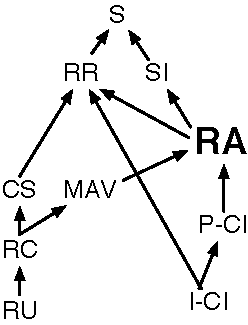
\includegraphics[width=1.3in]{diagram/isolation-graffle.pdf}
\end{center}
\caption{Comparison of RA with isolation levels
  from~\cite{adya,hat-vldb}. RU: Read Uncommitted, RC: Read
  Committed, CS: Cursor Stability, MAV: Monotonic Atomic View, ICI:
  Item Cut Isolation, PCI: Predicate Cut Isolation, RA: Read Atomic,
  SI: Snapshot Isolation, RR: Repeatable Read (Adya \textit{PL-2.99}), S:
  Serializable.}
\label{fig:isolation}
\end{figure}

\subsection{RA and Serializability}
\label{sec:ra-serializable}

When we began this work, we started by examining the use cases
outlined in Section~\ref{sec:motivation} and deriving a weak isolation
guarantee that would be sufficient to ensure their correct
execution. For general-purpose read-write transactions, RA isolation
may indeed lead to non-serializable (and possibly incorrect) database
states and transaction outcomes. Yet, as Section~\ref{sec:usage}
hints, there appears to be a broader ``natural'' pattern for which RA
isolation appears to provide an intuitive (even ``correct'')
semantics. In this section, we show that for transactions
with a particular property of their item read and item write sets, RA is, in
fact, serializable. We define this property, called the
\textit{read-subset-items-written (RSIW) property}, prove that transactions
obeying the RSIW property lead to serializable outcomes, and discuss
the implications of the RSIW property for the applications outlined in
Section~\ref{sec:motivation}.

Because our system model operates on multiple versions, we must make a
small refinement to our use of the term ``serializability''---namely,
we draw a distinction between serial and one-copy serializable
schedules, per Bernstein et al.~\cite{bernstein-book}. First, we say that two histories
$H_1$ and $H_2$ are \textit{view equivalent} if they contain the same
set of committed transactions and have the same operations and $DSG(H_1)$
and $DSG(H_2)$ have the same direct read dependencies. For
consistency with prior work, we say that $T_i$ \textit{reads from}
$T_j$ if $T_i$ directly read-depends on $T_j$. We say that a
transaction is \textit{read-only} if it does not contain write
operations and that a transaction is \textit{write-only} if it does
not contain read operations. In this section, we concern ourselves
with \textit{one-copy serializability}~\cite{bernstein-book}, which we
define using the previous definition of view equivalence.

\begin{definition}[One-Copy Serializability]
  A history is one-copy serializable if it is view equivalent to a serial
  execution of the transactions over a single logical copy of the
  database.
\end{definition}

The basic intuition behind the RSIW property is straightforward: under
RA isolation, if application developers use a transaction to bundle a
set of writes that should be observed together, any transactions that
read from the items that were written will, in fact, behave ``properly''---or
one-copy serializably. That is, for read-only and write-only transactions, if
each reading transaction only reads a subset of the items that another
write-only transaction wrote, then RA isolation is equivalent to
one-copy serializable isolation. Before proving that this behavior is
one-copy serializable, we can more precisely characterize this condition as
follows:

\begin{definition}[Read-Subset-Items-Written] A read-only transaction
  $T_r$ exhibits the \textit{Read-Subset-Items-Written} property if,
  whenever $T_r$ reads a version produced by a write-only transaction
  $T_w$, $T_r$ only reads items written to by $T_w$.
\end{definition}

For example, consider the following History~\ref{hist:rsw}:
\begin{eqnarray}
\label{hist:rsw}
T_1 & w(x_1); w(y_1)\\
T_2 & r(x_1); w(y_1)\nonumber\\
T_3 & r(x_1); r(z_\bot)\nonumber
\end{eqnarray}

Under History~\ref{hist:rsw}, $T_2$ exhibits the RSIW property because
it reads a version produced by transaction $T_1$ and its item read set
($\{x,y\}$) is a subset of $T_1$'s item write set ($\{x,y\}$). However,
$T_3$ does not exhibit the RSIW property because $i.)$ $T_3$ reads from
$T_1$ but $T_3$'s read set ($\{x,z\}$) is not a subset of $T_1$'s
write set ($\{x,y\}$) and $ii.)$, perhaps more subtly, $T_3$ reads
from both $T_1$ and $T_\bot$.

We say that a history $H$ containing read-only and write-only
transactions exhibits the RSIW property (or \textit{has RSIW}) if every read-only transaction
in $H$ exhibits the RSIW property.

This brings us to our main result in this section:

\begin{theorem}
\label{thm:rsw}
If a history $H$ containing read-only and write-only transactions
has RSIW and is valid under RA isolation, then
$H$ is one-copy serializable.
\end{theorem}

The proof of Theorem~\ref{thm:rsw} is by construction: given a history
$H$ has RSIW and is valid under RA isolation, we
describe how to derive an equivalent one-copy serial execution of the
transactions in $H$. We begin with the construction procedure, provide examples
of how to apply the procedure, then prove that the procedure
converts RSIW histories to their one-copy serial equivalents. We
provide the proof in Section~\ref{sec:rsiwproof}

\minihead{Utility} Theorem~\ref{thm:rsw} is helpful because it
provides a simple syntactic condition for understanding when RA will
provide one-copy serializable access. For example, we can apply this
theorem to our use cases from Section~\ref{sec:motivation}. In the
case of multi-entity update and read, if clients issue read-only and
write-only transactions that obey the RSIW property, their result sets
will be one-copy serializable. The RSIW property holds for
equality-based lookup of single records from an index (e.g., fetch
from the index and subsequently fetch the corresponding base tuple,
each of which was written in the same transaction (e.g., was
auto-generated upon insertion of the tuple into the base
relation). However, the RSIW property does not in the event of
multi-tuple reads, leading to less intuitive behavior. Specifically,
if two different clients trigger two separate updates to an index
entry, some clients may observe one update but not the other, and
other clients may observe the opposite behavior. In this case, the
RAMP protocols still provide a snapshot view of the database according
to the index(es)---that is, clients will never observe base data that
is inconsistent with the index entries---but nevertheless surface
non-serializable database states. Finally, for more general
materialized view accesses, point queries and bulk insertions have
RSIW.

As discussed in Section~\ref{sec:motivation}, in the case of indexes
and views, it is helpful to view each physical data structure (e.g.,
a CRDT~\cite{crdt} used to represent an index entry) as a
\textit{collection} of versions. In this case, the RSIW property
applies only if clients make modifications to the entire collection at
once (e.g., as in a \texttt{DELETE CASCADE} operation).

Coupled with an appropriate algorithm ensuring RA isolation, we can
ensure one-copy serializable isolation. This addresses a long-standing
concern with our work: why is RA somehow ``natural'' for these use
cases (but not necessarily all use cases)?  We have encountered
applications that do not require one-copy serializable access---such
as the mailbox unread message maintenance from
Section~\ref{sec:motivation} and, in some cases, index maintenance for
non-read-modify-write workloads---and therefore may safely violate
RSIW. However, we believe the RSIW property is a handy principle (or,
at the least, rule of thumb) for reasoning about applications of RA
isolation and the RAMP protocols.

Finally, the RSIW property is only a \textit{sufficient} condition for
one-copy serializable behavior under RA isolation. It is not
necessary---for example, there are several alternative sufficient
conditions to consider. As a natural extension, while RSIW only
pertains to pairs of read-only and write-only transactions, one might
consider allowing readers to observe multiple write transactions. For
example, consider the following history:
\begin{eqnarray}
\label{hist:rsw-multi-right}
T_1 & w(x_1); w(y_1)\\
T_2 & w(u_2); w(z_2)\nonumber\\
T_3 & r(x_1); r(z_2)\nonumber
\end{eqnarray}
History~\ref{hist:rsw-multi-right} is valid under RA and is also
one-copy serializable but does not have RSIW: $T_3$ reads from
\textit{two} transactions' write sets. However, consider the following
history:
\begin{eqnarray}
\label{hist:rsw-multi-wrong}
T_1: & w(x_1); w(y_1)\\
T_2: & w(u_2); w(z_2)\nonumber\\
T_3: & r(x_1); r(z_\bot)\nonumber\\
T_4: & r(x_\bot); r(z_2)\nonumber
\end{eqnarray}
History~\ref{hist:rsw-multi-wrong} is valid under RA, consists only of
read-only and write-only transactions, yet is no longer
one-copy serializable. $T_3$ observes, in effect, a one-copy serializable prefix
beginning with $T_\bot; T_1$ while $T_4$ observes a prefix beginning
with $T_\bot; T_2$. Neither $T_3$ nor $T_4$ observes the prefixes
$T_\bot; T_1; T_2$ or $T_\bot; T_2; T_1$.

Thus, while there may indeed be useful criteria beyond the RSIW
property that we might consider as a basis for one-copy serializable
execution under RA, we have observed RSIW to be the most intuitive and
useful thus far. One clear criteria is to search for schedules or
restrictions under RA with an acyclic Directed Serialization Graph (from
Appendix~\ref{sec:rsiwproof}). The reason why RSIW is so simple for
read-only and write-only transactions is that each read-only
transaction only reads from one other transaction and does not induce
any additional anti-dependencies. Combining reads and writes
complicates reasoning about the acyclicity of the graph.

This exercise touches upon an important
lesson in the design and use of weakly isolated systems: by
restricting the set of operations accessible to a user (e.g., RSIW
read-only and write-only transactions), one can often achieve more
scalable implementations (e.g., using weaker semantics)
\textit{without} necessarily violating existing abstractions (e.g.,
one-copy serializable isolation). While prior work often focuses on
restricting only operations (e.g., to read-only or write-only
transactions~\cite{eiger,divy-writeonly}, or stored
procedures~\cite{calvin,hstore,jones-dtxn}, or single-site
transactions~\cite{megastore}) or only semantics (e.g., weak isolation
guarantees~\cite{hat-vldb,eiger,explicit-socc}), we see
considerable promise in better understanding the intersection between
and combinations of the two. This is often subtle and almost always
challenging, but the results---as we found here---may be surprising.

 \subsection{System Model and Scalability}
\label{sec:sysmodel}

We consider databases that are partitioned, with the set of items in
the database spread over multiple servers. Each item has a single
logical copy, stored on a server---called the item's
\textit{partition}---whose identity can be calculated using the
item. Clients forward operations on each item to the item's partition,
where they are executed. In our examples, all data items have the null
value ($\bot$) at database initialization. In this section, we do not
model replication of data items within a partition; this can happen at
a lower level of the system than our discussion (see
Section~\ref{sec:replication}) as long as operations on each item are
linearizable~\cite{dcomp-book}.

\minihead{Scalability criteria} As we discussed in
Section~\ref{sec:ramp-motivation}, large-scale deployments often eschew
transactional functionality on the premise that it would be too
expensive or unstable in the presence of failure and degraded
operating
modes~\cite{ladis,tao,bigtable,pnuts,dynamo,helland-trans,2pc-scalability,espresso,rainbird}. Our
goal in this paper is to provide robust and scalable transactional
functionality, and, so we first define criteria for ``scalability'':

\vspace{.5em}\noindent Per Section~\ref{sec:model},
\textit{Coordination-free execution} ensures that one client's
transactions cannot cause another client's to block and that, if a
client can contact the partition responsible for each item in its
transaction, the transaction will eventually commit (or abort of its
own volition). This prevents one transaction from causing another to
abort---which is particularly important in the presence of partial
failures---and guarantees that each client is able to make useful
progress. Note that ``strong'' isolation models like serializability
and Snapshot Isolation require coordination and thus limit
scalability. Locking is an example of a non-coordination-free
implementation mechanism.\vspace{.5em}

Many applications can limit their data accesses to a single
partition via explicit data
modeling~\cite{gstore,espresso,megastore,helland-trans} or
planning~\cite{schism,pavlo-partition}. However, this is not always
possible. In the case of secondary indexing, there is a cost
associated with requiring single-partition updates (scatter-gather
reads), while, in social networks like Facebook and large-scale
hierarchical access patterns as in Rainbird~\cite{rainbird}, perfect partitioning of
data accesses is near-impossible. Accordingly:

\vspace{.5em}\noindent\textit{Partition independence} ensures that, in
order to execute a transaction, a client only contacts partitions for
data items that its transaction directly accesses. Thus, a partition
failure only affects transactions that access items contained on the
partition. This also reduces load on servers not directly involved in
a transaction's execution. In the literature, partition independence
for replicated data is also called \textit{replica
  availability}~\cite{hat-vldb} or \textit{genuine partial
  replication}~\cite{gpr}. Using a centralized validator or scheduler
for transactions is an example of a non-partition-independent
implementation mechanism.\vspace{.5em}

In addition to the above requirements, we limit the \textit{metadata
  overhead} of algorithms. There are many potential solutions for
providing atomic visibility that rely on storing prohibitive amounts
of state. We will attempt to minimize the \textit{metadata}---that is,
data that the transaction did not itself write but which is required
for correct execution. In our algorithms, we will specifically provide
constant-factor metadata overheads (\raps, \rapb) or else overhead
linear in transaction size (but independent of data size; \rapl). As
an example of a solution using prohibitive amounts of metadata, each
transaction could send copies of all of its writes to every partition
it accesses so that readers observe all of its writes by reading a
single item. This provides RA isolation but requires considerable
storage. Other solutions may require extra data storage proportional
to the number of servers in the cluster or, worse, the database size,
which we discuss in Related Work (Chapter~\ref{c.relatedwork}).




\section{RAMP Transaction Algorithms}
\label{sec:ramp-algorithm}

Given specifications for RA isolation and scalability, we present
algorithms for achieving both. For ease of understanding, we first
focus on providing read-only and write-only transactions with a ``last
writer wins'' overwrite policy, then subsequently discuss how to
perform read/write transactions. Our focus in this section is on
intuition and understanding; we defer all correctness and scalability
proofs to Section~\ref{sec:rampproofs}, providing salient details inline.

At a high level, RAMP transactions allow reads and writes to proceed
concurrently. This provides excellent performance but, in turn,
introduces certain race conditions that could cause undesirable
anomalies: one transaction might only read a subset of another
transaction's writes, violating RA (i.e., fractured reads might
occur). Instead of preventing this race (hampering scalability), RAMP
readers \textit{autonomously} detect the race (using metadata attached
to each data item) and fetch any missing, in-flight writes from their
respective partitions. To make sure that readers never have to wait
for writes to arrive at a partition, writers use a two-phase (atomic
commitment) protocol that ensures that once a write is visible to
readers on one partition, any other writes in the transaction are
present on and, if appropriately identified by version, readable from
their respective partitions.

In this section, we present three algorithms that provide a trade-off
between the amount of metadata required and the expected number of
extra reads to fetch missing writes. As discussed in
Section~\ref{sec:motivation}, while techniques like distributed
locking couple mutual exclusion with atomic visibility of writes, RAMP
transactions correctly control visibility but allow concurrent and
scalable execution.

\subsection{RAMP-Fast}
\label{sec:rapl}


\begin{figure}[t!]
\begin{center}
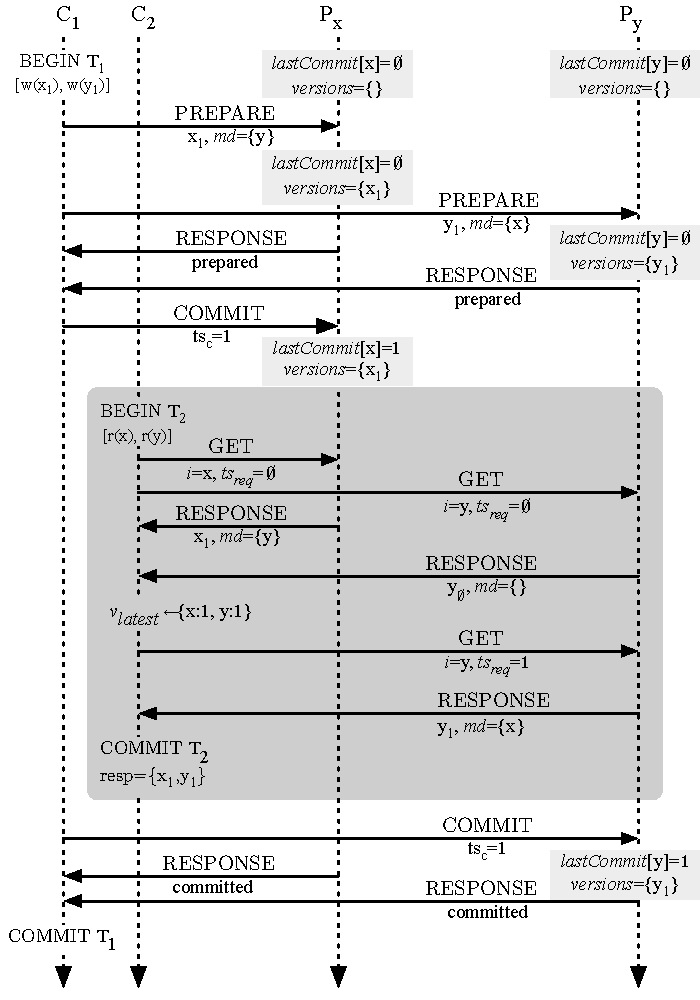
\includegraphics[width=.6\columnwidth]{diagram/rapl-big.pdf}\vspace{.5em}
\caption{Space-time diagram for \rapl execution for two transactions
  $T_1$ and $T_2$ performed by clients $C_1$ and $C_2$ on partitions
  $P_x$ and $P_y$. Lightly-shaded boxes represent current partition
  state ($lastCommit$ and $versions$), while the single darker box
  encapsulates all messages exchanged during $C_2$'s execution of
  transaction $T_2$.  Because $T_1$ overlaps with $T_2$, $T_2$ must
  perform a second round of reads to repair the fractured read between
  $x$ and $y$. $T_1$'s writes are assigned timestamp $1$. In our
  depiction, each item does not appear in its list of writes (e.g.,
  $P_x$ sees $\{y\}$ only and not $\{x,y\}$.}
\label{fig:rapl-execution}
\end{center}
\end{figure}

To begin, we present a RAMP algorithm that, in the race-free case,
requires one RTT for reads and two RTTs for writes, called
\texttt{RAMP-Fast} (abbreviated \rapl; Algorithm~\ref{alg:rapl}).
\rapl stores metadata in the form of write sets (overhead linear in
transaction size).

\minihead{Overview} Each write in \rapl
(lines~\ref{rapl-putall-start}--\ref{rapl-putall-end}) contains a
timestamp (line~\ref{rapl-newid}) that uniquely identifies the writing
transaction as well as a set of items written in the transaction
(line~\ref{rapl-metadata}). For now, combining a unique client ID and
client-local sequence number is sufficient for timestamp generation
(see also Section~\ref{sec:additional}).

\rapl write transactions proceed in two phases: a first round of
communication places each timestamped write on its respective
partition. In this \textsc{prepare} phase, each partition adds the
write to its local database ($versions$,
lines~\ref{rapl-versions},~\ref{rapl-beginprepare-client}--\ref{rapl-endprepare-client}). A
second round of communication
(lines~\ref{rapl-begincommit-client}--\ref{rapl-endcommit-client}) marks versions as committed. In this
\textsc{commit} phase, each partition updates an index containing the
highest-timestamped committed version of each item ($lastCommit$,
lines~\ref{rapl-lc},~\ref{rapl-begincommit-server}--\ref{rapl-endcommit-server}).

\rapl read transactions begin by first fetching the last
(highest-timestamped) committed version for each item from its
respective partition
(lines~\ref{rapl-client-firstround-start}--\ref{rapl-client-secondround-start}). Using
the results from this first round of reads, each reader can calculate
whether it is ``missing'' any versions (that is, versions that were
prepared but not yet committed on their partitions). The reader
calculates a mapping from each item $i$ to the highest timestamped
version of $i$ that appears in the metadata of any version (of $i$ or
of any other item) in the first-round read set
(lines~\ref{rapl-client-latest-start}--\ref{rapl-client-latest-end}). If
the reader has read a version of an item that has a lower timestamp
than indicated in the mapping for that item, the reader issues a
second read to fetch the missing version (by timestamp) from its
partition
(lines~\ref{rapl-client-secondround-start}--\ref{rapl-client-secondround-end}). Once
all missing versions are fetched (which can be done in parallel), the
client can return the resulting set of versions---the first-round
reads, with any missing versions replaced by the optional, second
round of reads.

\minihead{By example} Consider the \rapl execution depicted in
Figure~\ref{fig:rapl-execution}. $T_1$ writes to both $x$ and $y$,
performing the two-round write protocol on two partitions, $P_x$ and
$P_y$. However, $T_2$ reads from $x$ and $y$ while $T_1$ is
concurrently writing.  Specifically, $T_2$ reads from $P_x$
\textit{after} $P_x$ has committed $T_1$'s write to $x$, but $T_2$
reads from $P_y$ \textit{before} $P_y$ has committed $T_1$'s write to
$y$. Therefore, $T_2$'s first-round reads return $x=x_1$ and $y=\bot$,
and returning this set of reads would violate RA. Using the metadata
attached to its first-round reads, $T_2$ determines that it is missing
$y_1$ (since $v_{latest}[y]=1$ and $1 > \bot$) and so $T_2$
subsequently issues a second read from $P_y$ to fetch $y_1$ by
version. After completing its second-round read, $T_2$ can safely
return its result set. $T_1$'s progress is unaffected by $T_2$, and
$T_1$ subsequently completes by committing $y_1$ on $P_y$.



\minihead{Why it works} \rapl writers use metadata as a record of
intent: a reader can detect if it has raced with an in-progress commit
round and use the metadata stored by the writer to fetch the missing
data. Accordingly, \rapl readers only issue a second round of reads in
the event that they read from a partially-committed write transaction
(where some but not all partitions have committed a write). In this
event, readers will fetch the appropriate writes from the
not-yet-committed partitions. Most importantly, \rapl readers never
have to stall waiting for a write that has not yet arrived at a
partition: the two-round \rapl write protocol guarantees that, if a
partition commits a write, all of the corresponding writes in the
transaction are present on their respective partitions (though
possibly not committed locally). As long as a reader can identify the
corresponding version by timestamp, the reader can fetch the version
from the respective partition's set of pending writes without
waiting. To enable this, \rapl writes contain metadata linear in the
size of the writing transaction's write set (plus a timestamp per
write).\vspace{.5em}

\rapl requires two RTTs for writes: one for \textsc{prepare}
and one for \textsc{commit}. For reads, \rapl requires one RTT in the
absence of concurrent writes and two RTTs otherwise.

RAMP timestamps are only used to identify specific versions and in
ordering concurrent writes to the same item; \rapl transactions do not
require a ``global'' timestamp authority. For example, if
$lastCommit[k]=2$, there is no requirement that a transaction
with timestamp $1$ has committed or even that such a transaction
exists.

\begin{algorithm}[t!]
\small
\caption{RAMP-Fast}
\label{alg:rapl}
\newcommand{\myindent}{\hspace{-1em}}

\begin{algorithmic}[1]
\Statex{\textbf{\textit{Server-side Data Structures}}\\
$versions$: set of versions $\langle item, value,$ timestamp $ts_v,$ metadata $md\rangle$ \label{rapl-versions}\\
$lastCommit[i]$: last committed timestamp for item $i$\label{rapl-lc}}\vspace{.5em}

\Statex{\textbf{\textit{Server-side Methods}}}\vspace{.25em}

\Procedure{prepare}{$v$ : version}\label{rapl-beginprepare-server}
  \State $versions$.add($v$)\label{rapl-server-prepare}
  \State \Return
\EndProcedure\vspace{.5em}\label{rapl-endprepare-server}

\Procedure{commit}{$ts_c$ : timestamp}\label{rapl-begincommit-server}
  \State $I_{ts} \gets$ $\{w.item \mid w \in versions \wedge w.ts_v = ts_c\}$\label{rapl-server-commit-1}
  \State $\forall i \in I_{ts}$, $lastCommit[i] \gets
  \max(lastCommit[i], ts_c)$\label{rapl-server-commit-2}
\EndProcedure\vspace{.5em}\label{rapl-endcommit-server}

\Procedure{get}{$i$ : item, $ts_{req}$ : timestamp}\label{rapl-get-server-start}
  \If {$ts_{req} = \emptyset$\label{rapl-get-server-nots-start}}
  \State {\Return $v \in versions : v.item=i \wedge v.ts_v = lastCommit[item]$\label{rapl-get-server-nots-end}}
  \Else 
  \State {\Return $v \in versions : v.item = i \wedge  v.ts_v = ts_{req}$\label{rapl-get-server-withts-end}}
  \EndIf
\EndProcedure\label{rapl-get-server-end}
\Statex\hrulefill\vspace{.25em}

\Statex{\textbf{\textit{Client-side Methods}}}\vspace{.25em}

\Procedure{put\_all}{$W$ : set of $\langle item, value \rangle$}\label{rapl-putall-start}
  \State $ts_{tx} \gets$ generate new timestamp\label{rapl-newid}
  \State $I_{tx} \gets $ set of items in $W$\label{rapl-metadata}
  \ParFor{$\langle i, v\rangle \in W$}\label{rapl-beginprepare-client}
  \State $v \gets \langle item=i, value=v, ts_v=ts_{tx}, md=(I_{tx} - \{i\})\rangle$\label{rapl-prepare-data}
  \State\hspace{1em} invoke $\textsc{prepare}(v)$ on respective server (i.e., partition)\label{rapl-prepare-client}
  \EndParFor\label{rapl-endprepare-client}
  
  \ParFor{server $s : s$ contains an item in $W$}\label{rapl-begincommit-client}
  \State invoke $\textsc{commit}(ts_{tx})$ on $s$\label{rapl-commit-client}
  \EndParFor\label{rapl-endcommit-client}
\EndProcedure\vspace{.5em}\label{rapl-putall-end}

\Procedure{get\_all}{$I$ : set of items}\label{rapl-client-getall-start}
  \State $ret \gets \{\}$\label{rapl-client-firstround-start}
  \ParFor {$i \in I$}
  \State $ret[i] \gets \textsc{get}(i, \emptyset)$\label{rapl-client-firstround-get}
  \EndParFor\vspace{.25em}\label{rapl-client-firstround-end}

  \State $v_{latest} \gets \{\}$ (default value: $-1$)\label{rapl-client-latest-start}
  \For{response $r \in ret$}
  \For{$i_{tx} \in r.md$}
  \State $v_{latest}[i_{tx}] \gets \max(v_{latest}[i_{tx}], r.ts_v)$\label{rapl-client-latest-calculate}
  \EndFor
  \EndFor\vspace{.25em}\label{rapl-client-latest-end}

  \ParFor{item $i \in I$}\label{rapl-client-secondround-start}
  \If{$v_{latest}[i] > ret[i].ts_v$}\label{rapl-client-secondround-check}
  \State $ret[i] \gets \textsc{get}(i, v_{latest}[i])$\label{rapl-client-secondround-get}
  \EndIf
  \EndParFor\vspace{.25em}\label{rapl-client-secondround-end}

  \State \Return $ret$\label{rapl-client-getall-return}
\EndProcedure\label{rapl-client-getall-end}


\end{algorithmic}
\end{algorithm}


\subsection{RAMP-Small: Trading Metadata for RTTs}
\label{sec:raps}

\begin{figure}[t!]
\begin{center}
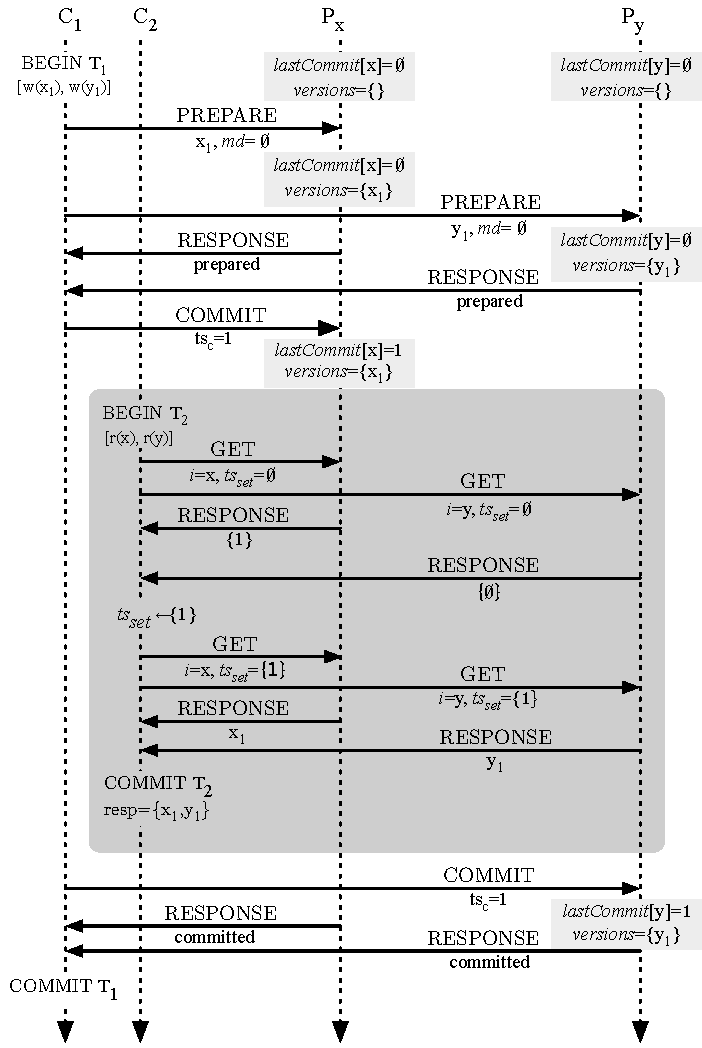
\includegraphics[width=.6\columnwidth]{diagram/raps-big.pdf}\vspace{.5em}
\caption{Space-time diagram for \raps execution for two transactions
  $T_1$ and $T_2$ performed by clients $C_1$ and $C_2$ on partitions
  $P_x$ and $P_y$. Lightly-shaded boxes represent current partition
  state ($lastCommit$ and $versions$), while the single darker box
  encapsulates all messages exchanged during $C_2$'s execution of
  transaction $T_2$. $T_1$ first fetches the highest committed
  timestamp from each partition, then fetches the corresponding
  version. In this depiction, partitions only return timestamps
  instead of actual versions in response to first-round reads.}
\label{fig:raps-execution}
\end{center}
\end{figure}

While \rapl requires metadata size linear in write set size but provides best-case
one RTT for reads, \texttt{RAMP-Small} (\raps) uses constant
metadata but always requires two RTT for reads
(Algorithm~\ref{alg:raps}). \raps and \rapl writes are identical, but,
instead of attaching the entire write set to each write, \raps writers
only store the transaction timestamp
(line~\ref{raps-prepare-data}). Unlike \rapl, \raps readers issue a
first round of reads to fetch the highest committed timestamp for each
item from its respective partition
(lines~\ref{raps-get-server-nots-end},~\ref{raps-client-firstround-start}--\ref{raps-client-firstround-end}). Then
the readers send the entire set of timestamps they received to
the partitions in a second round of communication
(lines~\ref{raps-client-secondround-start}--\ref{raps-client-secondround-end}). For
each item in the read request, \raps servers return the
highest-timestamped version of the item that also appears in the
supplied set of timestamps
(lines~\ref{raps-get-server-withts-start}--\ref{raps-get-server-withts-end}). Readers
subsequently return the results from the mandatory second round of
requests.

\minihead{By example} In Figure~\ref{fig:raps-execution}, under \raps,
$P_x$ and $P_y$ respectively return the sets $\{1\}$ and
$\{\bot\}$ in response to $T_2$'s first round of reads. $T_2$ would
subsequently send the set $\{1, \bot\}$ to both $P_x$ and $P_y$, which
would return $x_1$ and $y_1$.  (Including $\bot$ in the second-round
request is unnecessary, but we leave it in for ease of understanding.)

\minihead{Why it works} In \raps, if a transaction has committed on
some but not all partitions, the transaction timestamp will be
returned in the first round of any concurrent read transaction
accessing the committed partitions' items. In the (required) second
round of read requests, any prepared-but-not-committed partitions will
find the committed timestamp in the reader-provided set and return the
appropriate version. In contrast with \rapl, where readers explicitly
provide partitions with a specific version to return in the (optional)
second round, \raps readers defer the decision of which version to
return to the partition, which uses the reader-provided set to
decide. This saves metadata but increases RTTs, and the size of the
parameters of each second-round \textsc{get} request is (worst-case)
linear in the read set size. Unlike \rapl, there is no requirement to
return the value of the last committed version in the first round
(returning the version, $lastCommit[k]$, suffices in
line~\ref{raps-get-server-nots-end}).

\begin{algorithm}[t!]
\small
\caption{RAMP-Small}
\label{alg:raps}
\newcommand{\myindent}{\hspace{-1em}}
\begin{algorithmic}[1]
\Statex{\textbf{\textit{Server-side Data Structures}}}
\Statex same as in \rapl (Algorithm~\ref{alg:rapl}) \vspace{.5em}

\Statex{\textbf{\textit{Server-side Methods}}}\
\Statex \textsc{prepare}, \textsc{commit} same as in \rapl\vspace{.5em}

\Procedure{get}{$i$ : item, $ts_{set}$ : set of timestamps}\label{raps-get-server-start}
  \If{$ts_{set} = \emptyset$}
  \State \Return $v \in versions : v.item=i \wedge v.ts_v =
  lastCommit[k]$\label{raps-get-server-nots-end}
  \Else
  \State $ts_{match} = \{t \mid t \in ts_{set} \wedge \exists v \in versions : v.item = i \wedge v.t_v = t\}$\label{raps-get-server-withts-start}
  \State \Return $v \in versions : v.item = i \wedge  v.ts_v =
  max(ts_{match})$\label{raps-get-server-withts-end}
  \EndIf

\EndProcedure\label{raps-get-server-end}
\Statex\hrulefill\vspace{.25em}

\Statex{\textbf{\textit{Client-side Methods}}}\vspace{.25em}

\Procedure{put\_all}{$W$ : set of $\langle item, value \rangle$}
\Statex \hspace{1.5em} same as \rapl \textsc{put\_all} but do not instantiate $md$ on line~\ref{rapl-prepare-data}\label{raps-prepare-data}
\EndProcedure\vspace{.5em}\label{raps-putall-end}

\Procedure{get\_all}{$I$ : set of items}\label{raps-client-getall-start}
\State \hspace{.35em} $ts_{set} \gets \{\}$\label{raps-client-firstround-start}
\ParFor {$i \in I$}
    \State $ts_{set}.$add($\textsc{get}(i, \emptyset).ts_v$)\label{raps-client-firstround-get}
  \EndParFor\vspace{.25em}\label{raps-client-firstround-end}

  \State $ret \gets \{\}$
  \ParFor{item $i \in I$}\label{raps-client-secondround-start}
    \State $ret[i] \gets \textsc{get}(i, ts_{set})$ \label{raps-client-secondround-get}
  \EndParFor\vspace{.25em}\label{raps-client-secondround-end}

  \State \Return $ret$\label{raps-client-getall-return}
\EndProcedure\label{raps-client-getall-end}


\end{algorithmic}
\end{algorithm}

\subsection{RAMP-Hybrid: An Intermediate Solution}
\label{sec:rapb}

\texttt{RAMP-Hybrid} (\rapb; Algorithm~\ref{alg:rapb}) strikes a
compromise between \rapl and \raps. \rapb and \raps write protocols
are identical, but, instead of storing the entire write set (as in
\rapl), \rapb writers store a Bloom filter~\cite{bloomfilter}
representing the transaction write set
(line~\ref{rapb-putall-start}). \rapb readers proceed as in \rapl, with
a first round of communication to fetch the last-committed version of
each item from its partition
(lines~\ref{rapb-client-firstround-start}--\ref{rapb-client-firstround-end}). Given
this set of versions, \rapb readers subsequently compute a list of
\textit{potentially} higher-timestamped writes for each item
(lines~\ref{rapb-client-compute-start}--\ref{rapb-client-compute-end}). Any
potentially missing versions are fetched in a second round of reads
(lines~\ref{rapb-client-secondround-start}).

\minihead{By example} In Figure~\ref{fig:rapl-execution}, under \rapb,
$x_1$ would
contain a Bloom filter with positives for $x$ and $y$ and $y_{\bot}$
would contain an empty Bloom filter. $T_2$ would check for the
presence of $y$ in $x_1$'s Bloom filter (since $x_1$'s version is $1$
and $1 > \bot$) and, finding a match, conclude that it is potentially
missing a write ($y_1$). $T_2$ would subsequently fetch $y_1$ from
$P_y$.

\minihead{Why it works} \rapb is effectively a hybrid between \rapl
and \raps. If the Bloom filter has no false positives, \rapb reads
behave like \rapl reads. If the Bloom filter has all false positives,
\rapb reads behave like \raps reads. Accordingly, the number of
(unnecessary) second-round reads (i.e., which would not be performed
by \rapl) is controlled by the Bloom filter false positive rate, which
is in turn (in expectation) proportional to the size of the Bloom
filter. Any second-round \textsc{get} requests are accompanied by a
set of timestamps that is also proportional in size to the false
positive rate.  Therefore, \rapb exposes a trade-off between metadata
size and expected performance. To understand why \rapb is safe, we
simply have to show that any false positives (second-round reads) will
not compromise the integrity of the result set; with unique
timestamps, any reads due to false positives will return null.

\begin{algorithm}[t!]
\small
\caption{RAMP-Hybrid}
\label{alg:rapb}
\newcommand{\myindent}{\hspace{-1em}}
\begin{algorithmic}[1]
\Statex{\textbf{\textit{Server-side Data Structures}}}
\Statex same as in \rapl (Algorithm~\ref{alg:rapl}) \vspace{.5em}

\Statex{\textbf{\textit{Server-side Methods}}}\
\Statex \textsc{prepare}, \textsc{commit} same as in \rapl
\Statex \textsc{get} same as in \raps
\Statex\hrulefill\vspace{.25em}

\Statex{\textbf{\textit{Client-side Methods}}}\vspace{.25em}

\Procedure{put\_all}{$W$ : set of $\langle item, value \rangle$}~\label{rapb-putall-start}
\Statex \hspace{1.5em} same as \rapl \textsc{put\_all} but instantiate $md$ on line~\ref{rapl-prepare-data}
\Statex \hspace{1.5em} with Bloom filter containing $I_{tx}$
\EndProcedure\vspace{.5em}\label{rapb-putall-end}

\Procedure{get\_all}{$I$ : set of items}\label{rapb-client-getall-start}
  \State $ret \gets \{\}$\label{rapb-client-firstround-start}
  \ParFor {$i \in I$}
  \State $ret[i] \gets \textsc{get}(i, \emptyset)$\label{rapb-client-firstround-get}
  \EndParFor\vspace{.25em}\label{rapb-client-firstround-end}

  \State $v_{fetch} \gets \{\}$

  \For{version $v \in ret$}\label{rapb-client-compute-start}
  \For{version $v' \in ret: v' \neq v$}
  \If{$v.ts_v > v'.ts_v \wedge v.md.lookup(v'.item) \rightarrow True$}
    \State $v_{fetch}[v'.item]$.add($v.ts_v$)\label{rapb-client-compute-step}
  \EndIf
  \EndFor
  \EndFor\label{rapb-client-compute-end}

  \ParFor{item $i \in v_{fetch}$}\label{rapb-client-secondround-start}
        \State $ret[i] \gets \textsc{get}(k, v_{fetch}[i])$ \textbf{if}
        $\textsc{get}(k, v_{fetch}[i]) \neq \bot$ \label{rapb-client-secondround-get}
  \EndParFor\vspace{.25em}\label{rapb-client-secondround-start}
  \State \Return $ret$\label{rapb-client-getall-return}
\EndProcedure\label{rapb-client-getall-end}


\end{algorithmic}
\end{algorithm}


\subsection{Summary and Additional Details}

The RAMP algorithms allow readers to safely race writers without
requiring either to stall. The metadata attached to each write allows
readers in all three algorithms to safely handle concurrent and/or
partial writes and in turn allows a trade-off between metadata size
and performance (Table~\ref{table:rap-compare}): \rapl is optimized
for fast reads, \raps is optimized for small metadata, and \rapb is,
as the name suggests, a middle ground. \rapl requires metadata linear
in transaction size, while \raps and \rapb require constant
metadata. However, \raps and \rapb require more RTTs for reads
compared to \rapl when there is no race between readers and
writers. When reads and writes race, in the worst case, all algorithms
require two RTTs for reads.  Writes always require two RTTs to prevent
readers from stalling due to missing, unprepared writes.

RAMP algorithms are scalable because clients only contact partitions
directly accessed by their transactions (partition independence), and clients
cannot stall one another (are coordination-free). More
specifically, readers do not interfere with other readers, writers do
not interfere with other writers, and readers and writers can proceed
concurrently. When a reader races a writer to the same items, the
writer's new versions will only become visible to the reader (i.e., be
committed) once it is guaranteed that the reader will be able to fetch
all of them (possibly via a second round of communication). A reader
will \textit{never} have to stall waiting for writes to arrive at a
partition (for details, see Invariant~\ref{inv:suitable-present} in
the Appendix); however, the reader may have to contact the servers
twice in order to fetch any versions that were missing from its first
set of reads.


\begin{table}
\begin{center}
{
\begin{tabular}{|c|c|c|c|c|c|c|}
\hline
\multirow{2}{*}{\textbf{Algorithm}} & \multicolumn{3}{c|}{\textbf{RTTs/transaction}} & \multicolumn{2}{c|}{\textbf{Metadata (+stamp)}} \\
 & \multicolumn{1}{c}{W} & \multicolumn{1}{c}{R (stable)} & \multicolumn{1}{c|}{R ($O$)}& \multicolumn{1}{c}{\small Stored} & \multicolumn{1}{c|}{\small Per-Request}\\\hline

{ \rapl} & { 2 } & {1} & {2} & { txn items } & - \\
{ \raps} & { 2 } &  {2} & {2} & - & { stamp/item} \\
{ \rapb} & { 2 } & {$1+\epsilon$} & {2} & { Bloom filter} & { stamp/item}\\\hline
\end{tabular}}
\caption{Comparison of basic algorithms: RTTs required for writes (W),
  reads (R) without concurrent writes and in the worst case ($O$),
  stored metadata and metadata attached to read requests (in addition 
  to a timestamp for each). \label{table:rap-compare}}
\end{center}



\end{table}

\label{sec:additional}

Below, we discuss relevant implementation details.

\minihead{Multi-versioning and garbage collection} RAMP transactions
rely on multi-versioning to allow readers to access versions that have
not yet committed and/or have been overwritten. In our pseudocode, we
have presented an implementation based on multi-versioned storage; in
practice, multi-versioning can be implemented by using a
single-versioned storage engine for retaining the last committed
version of each item and using a ``look-aside'' store for access to
both prepared-but-not-yet-committed writes and (temporarily) any
overwritten versions. The look-aside store should make prepared
versions durable but can---at the risk of aborting transactions in the
event of a server failure---simply store any overwritten versions in
memory. Thus, with some work, RAMP algorithms are portable to non-multi-versioned storage systems.

In both architectures, each partition's data will grow without bound
if old versions are not removed. If a committed version of an item is
not the highest-timestamped committed version (i.e., a committed
version $v$ of item $k$ where $v < lastCommit[k]$), it can be safely
discarded (i.e., garbage collected, or GCed) as long as no readers
will attempt to access it in the future (via second-round \textsc{get}
requests). It is easiest to simply limit the running time of read
transactions and GC overwritten versions after a fixed amount of real
time has elapsed. Any read transactions that take longer than this GC
window can be restarted~\cite{cops,eiger}. Therefore, the maximum
number of versions retained for each item is bounded by the item's
update rate, and servers can reject any client \textsc{get} requests
for versions that have been GCed (and the read transaction can be
restarted). This violates availability under asynchronous network
behavior, so, as a fallback and a more principled solution, partitions
can also gossip the timestamps of items that have been overwritten and
have not been returned in the first round of any ongoing read
transactions. Under \rapl, if a second-round read request arrives a
server and the server does not have that version due to garbage
collection, it can safely ignore the request or signal failure.

\minihead{Read-write transactions} Until now, we have focused on
read-only and write-only transactions. However, we can extend our
algorithms to provide read-write transactions. If transactions
pre-declare the data items they wish to read, then the client can
execute a \textsc{get\_all} transaction at the start of transaction
execution to pre-fetch all items; subsequent accesses to those items
can be served from this pre-fetched set. Clients can buffer any writes
and, upon transaction commit, send all new versions to servers (in
parallel) via a \textsc{put\_all} request. As in
Section~\ref{sec:ra-def}, this may result in anomalies due to
concurrent update but does not violate RA isolation. Given the
benefits of pre-declared read/write
sets~\cite{schism,pavlo-partition,calvin} and write
buffering~\cite{spanner,f1}, we believe this is a reasonable
strategy. For secondary index lookups, clients can first look up
secondary index entries then subsequently (within the same
transaction) read primary data (specifying versions from index entries as
appropriate).

\minihead{Timestamps} Timestamps should be unique across transactions,
and, for ``session'' consistency (Appendix), increase on a per-client
basis. Given unique client IDs, a client ID and sequence number form
unique transaction timestamps without coordination. Without unique
client IDs, servers can assign unique timestamps with high probability
using UUIDs and by hashing transaction contents.

\minihead{Overwrites} In our algorithms, versions are overwritten
according to a highest-timestamp-wins policy. In practice, and, for
commutative updates, users may wish to employ a different policy upon
\textsc{commit}: for example, perform set union. In this case,
$lastCommit[k]$ contains an abstract data type (e.g., set of versions)
that can be updated with a $merge$
operation~\cite{dynamo,sessionguarantees} (instead of
$updateIfGreater$) upon commit. This treats each committed record as a
set of versions, requiring additional metadata (that can be GCed as in
Section~\ref{sec:optimizations}).


\subsection{Distribution and Fault Tolerance}
\label{sec:replication}

RAMP transactions operate in a distributed setting, which poses
challenges due to latency, partial failure, and network
partitions. Under coordination-free execution, failed clients do not
cause other clients to fail, while partition independence ensures that
clients only have to contact partitions for items in their
transactions. This provides fault tolerance and availability as long
as clients can access relevant partitions. In this section, we address
incident concerns. First, replication can be used to increase the
number of servers hosting a partition, thus increasing
availability. Second, we describe the RAMP protocol behavior when
clients are unable to contact servers.

\minihead{Replication} RAMP protocols can benefit from a variety of
mechanisms including traditional database master-slave replication
with failover, quorum-based protocols, and state machine replication,
which increase the number of physical servers that host a given data
item~\cite{bernstein-book}. To improve durability, RAMP clients can
wait until the effects of their operations (e.g., modifications to
\textit{versions} and \textit{lastCommit}) are persisted to multiple
physical servers before returning from \textsc{put\_all} calls (either
via master-to-slave replication or via quorum replication and by
performing two-phase commit across multiple active servers). Notably,
because RAMP transactions can safely overlap in time, replicas can
process different transactions' \textsc{prepare} and \textsc{commit}
requests in parallel. Availability can also benefit in many protocols,
such as quorum replication. We discuss more advanced replication
techniques in Section~\ref{sec:multidc}.

\minihead{Stalled Operations} RAMP writes use a two-phase atomic
commitment protocol that ensures readers never block waiting for
writes to arrive. As discussed in Section~\ref{sec:motivation}, every
ACP may block during failures~\cite{bernstein-book}. However, under 
coordination-free execution, a blocked transaction (due to failed
clients, failed servers, or network partitions) cannot cause other
transactions to block. Stalled writes act only as ``resource
leaks'' on partitions: partitions will retain prepared versions
indefinitely unless action is taken.

To ``free'' these leaks, RAMP servers can use the Cooperative
Termination Protocol (CTP) described in~\cite{bernstein-book}. CTP can
always complete the transaction except when every partition has
performed \textsc{prepare} but no partition has performed
\textsc{commit}. In CTP, if a server $S_p$ has performed
\textsc{prepare} for transaction $T$ but times out waiting for a
\textsc{commit}, $S_p$ can check the status of $T$ on any other
partitions for items in $T$'s write set. If another server $S_c$ has
received \textsc{commit} for $T$, then $S_p$ can \textsc{commit}
$T$. If $S_a$, a server responsible for an item in $T$, has not
received \textsc{prepare} for $T$, $S_a$ and $S_p$ can promise never
to \textsc{prepare} or \textsc{commit} $T$ in the future and $S_p$ can
safely discard its versions.  Under CTP, if a client blocks
mid-\textsc{commit}, the servers will ensure that the writes will
eventually \textsc{commit} and therefore become visible on all
partitions. A client recovering from a failure can read from the
servers to determine if they unblocked its write.

CTP only runs when writes
block (or time-outs fire) and runs \textit{asynchronously} with
respect to other operations. CTP requires that \textsc{prepare}
messages contain a list of servers involved in the transaction (a
subset of \rapl metadata but a superset of \rapb and \raps) and that
servers remember when they \textsc{commit} and ``abort'' writes (e.g.,
in a log file). Compared to alternatives (e.g., replicating
clients~\cite{paxos-commit}), we have found CTP to be both lightweight
and effective. We evaluate CTP in Section~\ref{sec:ctp}.

\subsection{Additional Semantics}
\label{sec:ramp-semantics}

While our RAMP transactions provide RA isolation, they also provide a
number of additional useful guarantees. With linearizable servers,
once a user's operation completes, all other users will observe its
effects (regular register semantics, applied at the transaction
level); this provides a notion of real-time recency. This also ensures
that each user's operations are visible in the order in which they are
committed. Our RAMP implementations provide a variant of PRAM
consistency, where, for each item, each user's writes are
serialized~\cite{pram} (i.e., ``session''
ordering~\cite{daudjee-session}). For example, if a user updates her
privacy settings and subsequently posts a new photo, the photo cannot
be read without the privacy setting change~\cite{pnuts}. However, PRAM
does not respect the \textit{happens-before}
relation~\cite{lamportclocks} across users (or missing dependencies, as
discussed in Section~\ref{sec:ra-compare}). If Sam reads Mary's
comment and replies to it, other users may read Sam's comment without
Mary's comment. We further discuss this issue in
Section~\ref{sec:causal}.

\subsection{Further Optimizations}
\label{sec:optimizations}

\noindent RAMP algorithms also allow several possible optimizations:

\minihead{Faster commit detection} If a server returns a version in
response to a \textsc{get} request, then the transaction that created
the version must have issued a \textsc{commit} on at least one
server. In this case, the server can safely mark the version as
committed and update $lastCommit$. This means that the transaction
commit will be reflected in any subsequent \textsc{get} requests that
read from $lastCommit$ for this item---even though the \textsc{commit}
message from the client may yet be delayed. The net effect is that the
later \textsc{get} requests may not have to issue second-round reads
to fetch the versions that otherwise would not have been marked as
committed. This scenario will occur when all partitions have performed
\textsc{prepare} and at least one server but not all partitions have
performed \textsc{commit} (as in CTP). This allows faster updates to
$lastCommit$ (and therefore fewer expected \rapl and \rapb RTTs).

\minihead{Metadata garbage collection} Once all of transaction $T$'s
writes are committed on each respective partition (i.e., are reflected in
$lastCommit$), readers are guaranteed to read $T$'s writes (or later
writes). Therefore, non-timestamp metadata for $T$'s writes stored in
\rapl and \rapb (write sets and Bloom filters) can be
discarded. Detecting that all servers have performed \textsc{commit}
can be performed asynchronously via a third round of communication
performed by either clients or servers.

\minihead{One-phase writes} We have considered two-phase writes, but,
if a user does not wish to read her writes (thereby sacrificing
session guarantees outlined in Section~\ref{sec:ramp-semantics}), the
client can return after issuing its \textsc{prepare} round (without
sacrificing durability). The client can subsequently execute the
\textsc{commit} phase asynchronously, or, similar to optimizations
presented in Paxos Commit~\cite{paxos-commit}, the servers can
exchange \textsc{prepare} acknowledgments with one another and decide
to \textsc{commit} autonomously. This optimization is safe because
multiple \textsc{prepare} phases can safely overlap. We leverage a
similar observation in Section~\ref{sec:multidc}.



\section{Experimental Evaluation}
\label{sec:evaluation}
\label{sec:ramp-evaluation}

We proceed to experimentally demonstrate RAMP transaction scalability
as compared to existing transactional and non-transactional
mechanisms. \rapl, \rapb, and often \raps outperform existing
solutions across a range of workload conditions while exhibiting
overheads typically within $8\%$ and no more than $48\%$ of peak
throughput. As expected from our theoretical analysis, the performance
of our RAMP algorithms does not degrade substantially under contention
and scales linearly to over $7.1$ million operations per second on
$100$ servers. These outcomes validate our goal of coordination-free
design.

\subsection{Experimental Setup}
\label{sec:setup}

To demonstrate the effect of concurrency control on performance and
scalability, we implemented several concurrency control algorithms in
a partitioned, multi-versioned, main-memory database prototype. Our
prototype is in Java and employs a custom RPC system for
serialization. Servers are arranged as a distributed hash
table~\cite{chord} with partition placement determined by random
hashing of keys to servers. As in stores like Dynamo~\cite{dynamo},
clients can connect to any server to execute operations, which the
server will perform on their behalf (i.e., each server acts as a
client in our RAMP pseudocode). We implemented \rapl, \raps, and \rapb
and configure a wall-clock GC window of $5$ seconds as described in
Section~\ref{sec:additional}. \rapb uses a $256$-bit Bloom filter
based on an implementation of MurmurHash2.0~\cite{murmurhash}, with
four hashes per entry; to demonstrate the effects of filter
saturation, we do not modify these parameters in our experiments. Our
prototype utilizes the faster commit detection optimization from
Section~\ref{sec:additional}. We chose not to employ metadata garbage
collection and one-phase writes in order to preserve session
guarantees and because metadata overheads were generally minor.

\minihead{Algorithms for comparison} As a baseline, we do not employ
any concurrency control (denoted \nwnr, for no write and no read
locks); reads and writes take one RTT and are executed in parallel.

We also consider three lock-based mechanisms~\cite{gray-isolation}: long write locks and
long read locks, providing Repeatable Read
isolation (\textit{PL-2.99}; denoted \lwlr), long write locks with short read
locks, providing Read Committed isolation (\textit{PL-2L}; denoted
\lwsr; does not provide RA), and long write locks with no read locks,
providing Read Uncommitted isolation (\lwnr;
also does not provide RA). While only \lwlr provides RA, \lwsr and
\lwnr provide a useful basis for comparison, particularly in measuring
concurrency-related locking overheads. To avoid deadlocks, the system
lexicographically orders lock requests by item and performs them
sequentially. When locks are not used (as for reads in \lwnr and reads
and writes for \nwnr), the system parallelizes operations.

We also consider an algorithm where, for each transaction, designated
``coordinator'' servers enforce RA isolation---effectively, the Eiger
system's 2PC-PCI mechanism~\cite{eiger} (denoted \mstr;
Chapter~\ref{c.relatedwork}). Writes proceed via prepare and commit
rounds, but any reads that arrive at a partition and while a write
transaction to the same item is pending must contact a (randomly chosen,
per-write-transaction) ``coordinator'' partition to determine whether
the coordinator's prepared writes have been committed. Writes require
two RTTs, while reads require one RTT during quiescence and two RTTs
in the presence of concurrent updates (to a variable number of
coordinator partitions---linear in the number of concurrent writes to
the item). Using a coordinator violates partition independence
but---in this case---is still coordination-free. We optimize 2PC-PCI reads by having
clients determine a read timestamp for each transaction (eliminating
an RTT) and do not include happens-before metadata.

This range of lock-based strategies (\lwnr, \lwsr, \lwnr), recent
comparable approach (\mstr), and best-case (\nwnr; no concurrency
control) baseline provides a spectrum of strategies for comparison.

% espresso: 1000:1, f1 via spanner: 

\minihead{Environment and benchmark} We evaluate each algorithm using
the YCSB benchmark~\cite{ycsb} and deploy variably-sized sets of
servers on public cloud infrastructure. We employ \texttt{cr1.8xlarge}
instances on Amazon EC2 and, by default, deploy five partitions on
five servers. We group sets of reads and sets of writes into read-only
and write-only transactions (default size: 4 operations), and use the
default YCSB workload (\texttt{workloada}, with Zipfian distributed
item accesses) but with a 95\% read and 5\% write proportion, reflecting
read-heavy applications
(Section~\ref{sec:motivation},~\cite{tao,eiger,rainbird}; e.g., Tao's
500 to 1 reads-to-writes~\cite{tao,eiger}, Espresso's 1000 to 1
Mailbox application~\cite{espresso}, and Spanner's 3396 to 1
advertising application~\cite{spanner}).

By default, use $5000$ YCSB clients distributed across 5 separate EC2
instances. As in stock YCSB, each client makes a sequence of
synchronous requests to the database. When we later vary the number of
clients, we keep the number of servers hosting the clients fixed. To
fully expose our metadata overheads, use a value size of 1 byte per
write. We found that lock-based algorithms were highly inefficient for
YCSB's default 1000 item database, so we increased the database size
to one million items by default to decrease contention. Each version
contains a timestamp ($64$ bits), and, with YCSB keys (i.e., item IDs)
of size 11 bytes and a transaction length $L$, \rapl requires 11$L$
bytes of metadata per version, while \rapb requires 32 bytes. We
successively vary several parameters, including number of clients,
read proportion, transaction length, value size, database size, and
number of servers and report the average of three sixty-second trials.

\subsection{Experimental Results: Comparison}
\label{sec:eval-compare}

Our first set of experiments focuses on two metrics: performance
compared to baseline and performance compared to existing
techniques. The overhead of RAMP algorithms is typically less than
8\% compared to baseline (\nwnr) throughput, is sometimes zero, and
is never greater than 50\%. \rapl and \rapb always outperform the
lock-based and \mstr techniques, while \raps outperforms lock-based
techniques and often outperforms \mstr. We proceed to demonstrate this
behavior over a variety of conditions:



\minihead{Number of clients} RAMP performance scales well with
increased load and incurs little overhead
(Figure~\ref{fig:clients}). With few concurrent clients, there are few
concurrent updates and therefore few second-round reads; performance
for \rapl and \rapb is close to or even matches that of \nwnr. At peak
throughput with 10,000 clients, \rapl and \rapb pay a throughput
overhead of 4.2\% compared to \nwnr. \rapl and \rapb exhibit
near-identical performance; the \rapb Bloom filter triggers few false
positives and therefore few extra RTTs compared to \rapl. \raps
incurs greater overhead and peaks at almost 60\% of the throughput
of \nwnr. Its guaranteed two-round trip reads are expensive and it
acts as an effective lower bound on \rapl and \rapb performance. In
all configurations, the algorithms achieve low latency. \rapl, \rapb,
\nwnr less than 35~ms on average and less than 10~ms at 5,000
clients; \raps less than 53~ms, 14.3~ms at 5,000 clients.



In comparison, the remaining algorithms perform less favorably. In
contrast with the RAMP algorithms, \mstr servers must check a
coordinator server for each in-flight write transaction to determine
whether to reveal writes to clients. For modest load, the overhead of
these commit checks places \mstr performance between that of \raps and
\rapb.  Under YCSB's Zipfian workload, there is a high probability
that the several ``hot'' keys in the workload have a pending write,
requiring a \mstr commit check. The number of in-flight writes further
increases with load, increasing the number of \mstr commit
checks. This in turn decreases throughput, and, with 10,000 concurrent
clients, \mstr performs so many commit checks per read that it
underperforms the \lwnr lock-based scheme. Under this configuration,
more than 20\% of reads trigger a commit check, and, on servers with
hot items, each commit check requires indirected coordinator checks
for an average of 9.84 transactions. Meanwhile, multi-partition
locking is expensive~\cite{pavlo-partition}: with 10,000 clients, the
most efficient algorithm, \lwnr, attains only 28.6\% of the
throughput of \nwnr, while the least efficient, \lwlr, attains only
1.6\% and peaks at 3,412 transactions per second.


\begin{figure}[th!]
\begin{center}
{
\includegraphics[width=\textwidth]{figs/legend-oneline.pdf}\vspace{0em}}
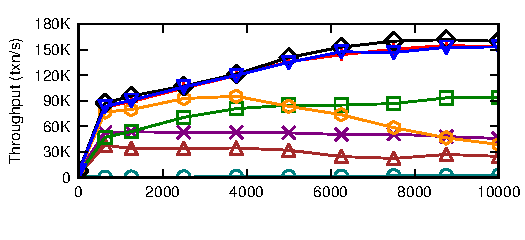
\includegraphics[width=.65\columnwidth]{figs/threads-thru.pdf}\vspace{-2em}
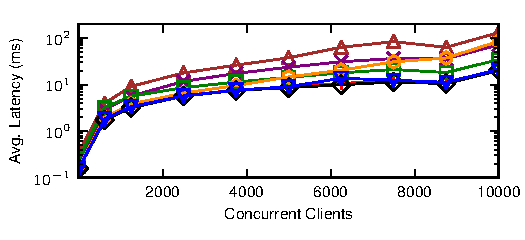
\includegraphics[width=.65\columnwidth]{figs/threads-lat.pdf}
\end{center}\vspace{-.5em}
\caption{Throughput and latency under varying client load. We omit
  latencies for \lwlr, which peaked at over 1.5s.}
\label{fig:clients}
\end{figure}


\begin{figure}[th!]
\begin{center}

\includegraphics[width=\textwidth]{figs/legend-oneline.pdf}\vspace{0em}
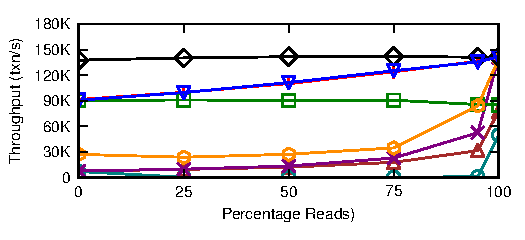
\includegraphics[width=.65\columnwidth]{figs/rprop-thru.pdf}\vspace{-1em}
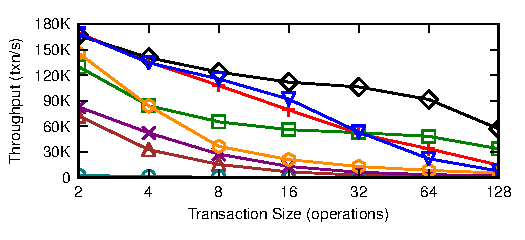
\includegraphics[width=.65\columnwidth]{figs/txnlen-thru.pdf}\vspace{-1em}
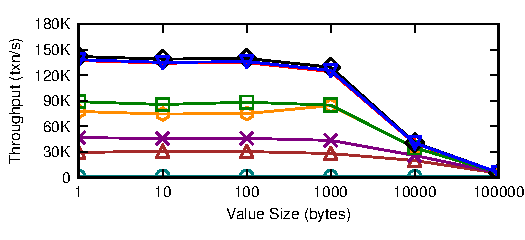
\includegraphics[width=.65\columnwidth]{figs/valuesize-thru.pdf}\vspace{-1em}
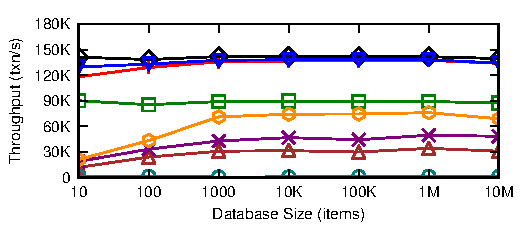
\includegraphics[width=.65\columnwidth]{figs/numkeys-thru.pdf}
\end{center}
\caption{Algorithm performance across varying workload
  conditions. \rapl and \rapb exhibit similar performance to \nwnr
  baseline, while \raps's 2 RTT reads incur a greater performance penalty
  across almost all configurations. RAMP transactions consistently
  outperform RA isolated alternatives.}
\label{fig:others}
\end{figure}

We subsequently varied several other workload parameters, which we
discuss below and plot in Figure~\ref{fig:others}:

\minihead{Read proportion} Increased write activity leads to a greater
number of races between reads and writes and therefore additional
second-round RTTs for \rapl and \rapb reads. With all write
transactions, all RAMP algorithms are equivalent (two RTT) and achieve
approximately 65\% of the throughput of \nwnr. With all reads, \rapl,
\raps, \nwnr, and \mstr are identical, with a single RTT. Between
these extremes, \rapl and \raps scale near-linearly with the write
proportion. In contrast, lock-based protocols fare poorly as
contention increases, while \mstr again incurs penalties due to commit
checks.


\minihead{Transaction length} Increased transaction lengths have
variable impact on the relative performance of RAMP
algorithms. Coordination-free execution ensures long-running
transactions are not penalized, but, with longer transactions,
metadata overheads increase. \rapl relative throughput decreases due
to additional metadata (linear in transaction length) and \rapb
relative performance also decreases as its Bloom filters
saturate. (However, YCSB's Zipfian-distributed access patterns result
in a non-linear relationship between length and throughput.) As
discussed above, we explicitly decided not to tune \rapb Bloom filter
size, but a logarithmic increase in filter size could improve \rapb
performance for large transaction lengths (e.g., 1024 bit filters
should lower the false positive rate for transactions of length 256
from over 92\% to slightly over 2\%).

\minihead{Value size} Value size similarly does not seriously impact
relative throughput. At a value size of 1B, \rapl is within 2.3\% of
\nwnr. However, at a value size of 100KB, \rapl performance nearly
matches that of \nwnr: the overhead due to metadata decreases, and
write request rates slow, decreasing concurrent writes (and
subsequently second-round RTTs). Nonetheless, absolute throughput
drops by a factor of 24 as value sizes moves from 1B to 100KB\@.

\minihead{Database size} RAMP algorithms are robust to high contention
for a small set of items: with only 1000 items in the database, \rapl
achieves throughput within 3.1\% of \nwnr. RAMP algorithms are
largely agnostic to read/write contention, although, with fewer items
in the database, the probability of races between readers and
in-progress writers increases, resulting in additional second-round
reads for \rapl and \rapb. In contrast, lock-based algorithms fare
poorly under high contention, while \mstr indirected commit checks
again incurred additional overhead. By relying on clients (rather than
additional partitions) to repair fractured writes, \rapl, \rapb, and
\raps performance is less affected by hot items. \vspace{.5em}

Overall, \rapl and \rapb exhibit performance close to that of no
concurrency control due to their independence properties and
guaranteed worst-case performance. As the proportion of writes
increases, an increasing proportion of \rapl and \rapb operations take
two RTTs and performance trends towards that of \raps, which provides
a constant two RTT overhead. In contrast, lock-based protocols perform
poorly under contention while \mstr triggers more commit checks than
\rapl and \rapb trigger second round reads (but still performs well
without contention and for particularly read-heavy workloads). The
ability to allow clients to independently verify read sets enables
good performance despite a range of (sometimes adverse) conditions
(e.g., high contention).


\begin{comment}
\begin{figure*}
\begin{center}

\includegraphics[width=.9\textwidth]{figs/legend-oneline.pdf}
\begin{minipage}[b]{0.49\linewidth}
\centering
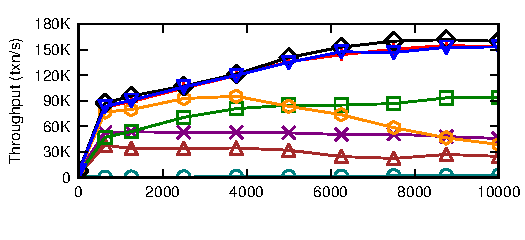
\includegraphics[width=\textwidth]{figs/threads-thru.pdf}
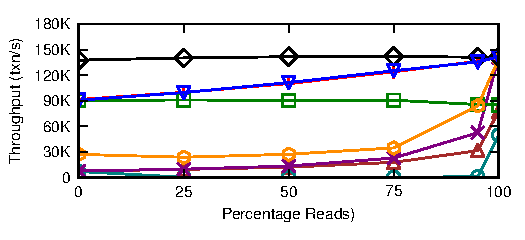
\includegraphics[width=\textwidth]{figs/rprop-thru.pdf}
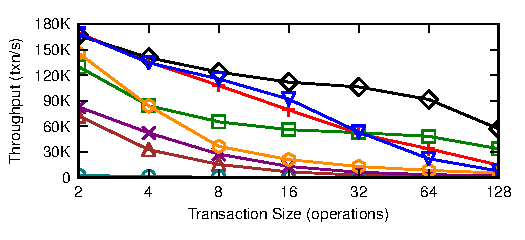
\includegraphics[width=\textwidth]{figs/txnlen-thru.pdf}
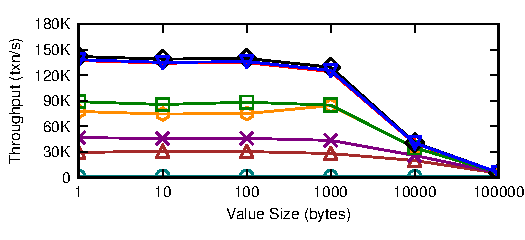
\includegraphics[width=\textwidth]{figs/valuesize-thru.pdf}
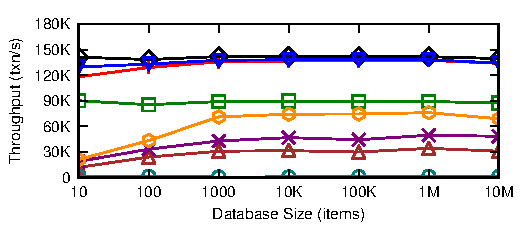
\includegraphics[width=\textwidth]{figs/numkeys-thru.pdf}
\end{minipage}
\begin{minipage}[b]{0.49\linewidth}
\centering
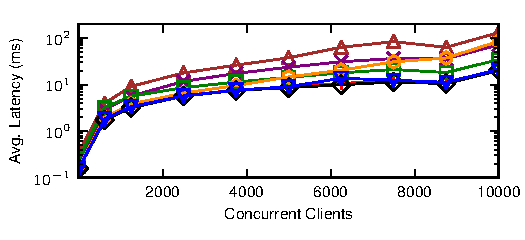
\includegraphics[width=\textwidth]{figs/threads-lat.pdf}
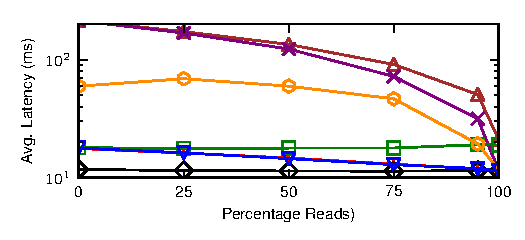
\includegraphics[width=\textwidth]{figs/rprop-lat.pdf}
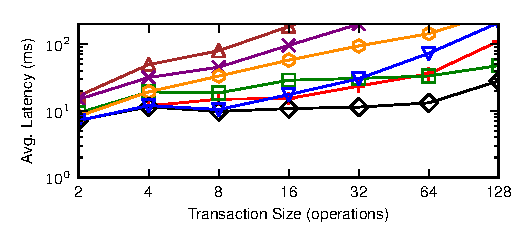
\includegraphics[width=\textwidth]{figs/txnlen-lat.pdf}
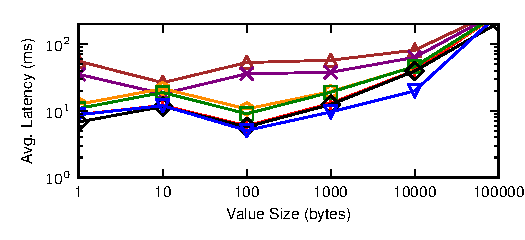
\includegraphics[width=\textwidth]{figs/valuesize-lat.pdf}
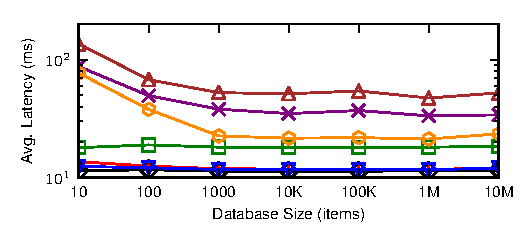
\includegraphics[width=\textwidth]{figs/numkeys-lat.pdf}
\end{minipage}
\end{center}
\caption{Comparison of algorithms for default parameters, sweeping one
  parameter per experiment}
\label{fig:comparison}

\end{figure*}
\end{comment}

\FloatBarrier
\subsection{Experimental Results: CTP Overhead} 
\label{sec:ctp}

We also evaluated the overhead of blocked writes in our implementation
of the Cooperative Termination Protocol discussed in
Section~\ref{sec:replication}. To simulate blocked writes, we
artificially dropped a percentage of \textsc{commit} commands in
\textsc{put\_all} calls such that clients returned from writes early
and partitions were forced to complete the commit via CTP. This
behavior is worse than expected because ``blocked'' clients continue
to issue new operations. The table below reports the throughput
reduction as the proportion of blocked writes increases (compared to
no blocked writes) for a workload of 100\% \rapl write
transactions:
\begin{center}
\small 
\begin{tabular}{|l|c|c|c|c|}
\hline
\textbf{Blocked \%} & 0.01\% & 0.1\% & 25\% & 50\% \\\hline
{\textbf{Throughput}} & No change & 99.86\% & 77.53\% & 67.92\% \\\hline
\end{tabular}
\end{center}
As these results demonstrate, CTP can reduce throughput because each
commit check consumes resources (namely, network and CPU
capacity). However, CTP only performs commit checks in the event of
blocked writes (or time-outs; set to 5s in our experiments), so a modest
failure rate of $1$ in $1000$ writes has a limited effect. The higher
failure rates produce a near-linear throughput reduction but, in
practice, a blocking rate of even a few percent is likely indicative
of larger systemic failures. As Figure~\ref{fig:others} hints, the
effect of additional metadata for the participant list in \rapb and
\raps is limited, and, for our default workload of 5\% writes,
we observe similar trends but with throughput degradation of 10\% or
less across the above configurations. This validates our initial motivation
behind the choice of CTP: average-case overheads are small.

\subsection{Experimental Results: Scalability}



\begin{figure}[th!]
\begin{center}
\hspace{5mm}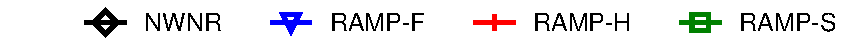
\includegraphics[width=\defaultfigwidth]{figs/legend-scaleout.pdf}\vspace{-.5em}
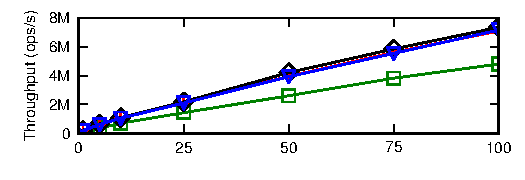
\includegraphics[width=.65\columnwidth]{figs/ns-thru.pdf}\vspace{-1.5em}
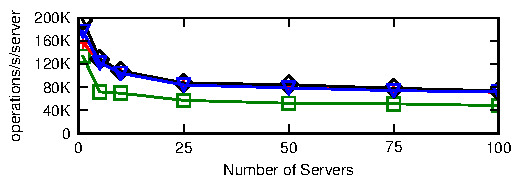
\includegraphics[width=.65\columnwidth]{figs/ns-perserver-thru.pdf}
\end{center}
\caption{RAMP transactions scale linearly to over $7$ million
  operations/s with comparable performance to \nwnr baseline.}
\label{fig:scaleout}
\end{figure}


We finally validate our chosen scalability criteria by demonstrating
linear scalability of RAMP transactions to 100 servers. We deployed an
increasing number of servers within the \texttt{us-west-2} EC2 region
and, to mitigate the effects of hot items during scaling, configured
uniform random access to items. We were unable to include more than 20
instances in an EC2 ``placement group,'' which guarantees 10 GbE
connections between instances, so, past 20 servers, servers
communicated over a degraded network. At around 40 servers, we
exhausted the \texttt{us-west-2b} ``availability zone'' (datacenter)
capacity and had to allocate our instances across the remaining zones,
further degrading network performance. To avoid bottlenecks on the
client, we deploy as many instances to host YCSB clients as we do to
host prototype servers.However, as shown in Figure~\ref{fig:scaleout},
each RAMP algorithm scales linearly. In expectation, at 100 servers,
almost all transactions span multiple servers: all but one in 100M
transactions is a multi-partition operation, highlighting the
importance of partition independence. With 100 servers, \rapl achieves
slightly under $7.1$ million operations per second, or 1.79 million
transactions per second on a set of 100 servers (71,635 operations
per partition per second). At all scales, \rapl throughput was always
within $10\%$ of \nwnr. With 100 servers, \rapl was within 2.6\%,
\raps within 3.4\%, and \raps was within 45\% of \nwnr. In light of
our scalability criteria, this behavior is unsurprising.

\FloatBarrier



\section{Applying and Modifying the RAMP Protocols}
\label{sec:ramp-application}

In this section, we discuss modifications to RAMP to enable multi-datacenter and efficient quorum replication as well as causally consistent operation. Our goals here are two-fold. First, we believe this section will be beneficial to systems implementers integrating RAMP protocols into databases such as Cassandra~\cite{cassandra-sigmod} that support wide-area and quorum-replicated deployments. Indeed, its inclusion is a reflection on many helpful reader comments asking for clarification on this topic. Second, we believe this material is a useful inclusion for readers who are familiar with existing and recent work on both multi-datacenter and causally consistent replication. Namely, RAMP is compatible with many of these replication scenarios, and, in some cases, enables new optimizations.

\subsection{Multi-Datacenter RAMP}
\label{sec:multidc}

The RAMP algorithms presented in this work have assumed linearizable server operation. Hence, if RAMP is used in a system where data items are replicated, then a linearizable replication mechanism must be used, such as a primary-backup or other replicated state machine approach. While this has simplified our discussion and results in reasonable performance in many environments, the cost of linearizability is often be expensive, particularly in geo-replicated environments where latency is lower-bounded by the speed of light~\cite{hat-vldb,pacelc}. While the RAMP algorithms' lack of coordination mitigates throughput penalties due to, for example, stalls during contended multi-partition access, actually accessing the partitions themselves may take time and increase the latency of individual operations. Moreover, in the event of partial failures, it is often beneficial to provide greater availability guarantees.

In this section, we discuss strategies for lowering the latency and improving the availability of operations. Our primary target in this setting is a multi-datacenter, geo-replicated context, where servers are located in separate clusters in possibly geographically remote regions. This setting has received considerable attention in recent research and, increasingly, in some of the largest production data management systems~\cite{walter,cops,eiger,spanner}. The actual porting of concurrency control algorithms to this context is not terribly difficult, but any inefficiencies due to synchronization and coordination are magnified in this setting, making it an idea candidate for practical study. Thus, we couch our discussion in the context of fully-replicated, geo-distributed clusters (i.e., groups of replicas of each partition).

The key challenge in achieving higher availability and lower latency in RAMP is ensuring that partially committed writes can still be completed. In the standard RAMP algorithms, this is accomplished by waiting to commit until after all partitions have prepared. Yet, in a replicated context, this waiting is potentially expensive; over wide-area networks, this can take hundreds of milliseconds. There are two straightforward ways to circumvent these overheads: deferring the commit operation and maintaining stickiness.


\begin{figure}[th!]
\begin{center}
\subfigure[High availability multi-cluster RAMP] {
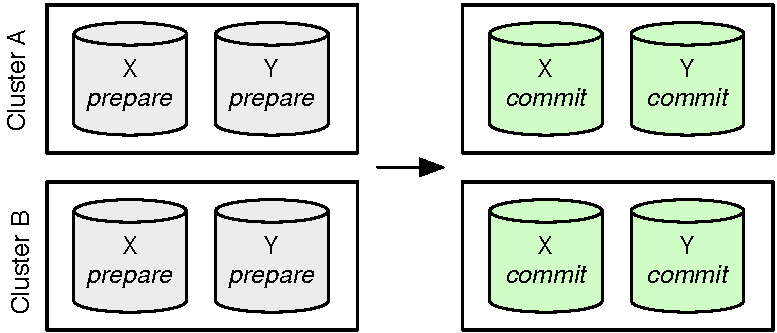
\includegraphics[width=.5\columnwidth]{diagram/mdc-ha.pdf}
\label{fig:mdc-ha}
}\\
\subfigure[Sticky multi-cluster RAMP] {
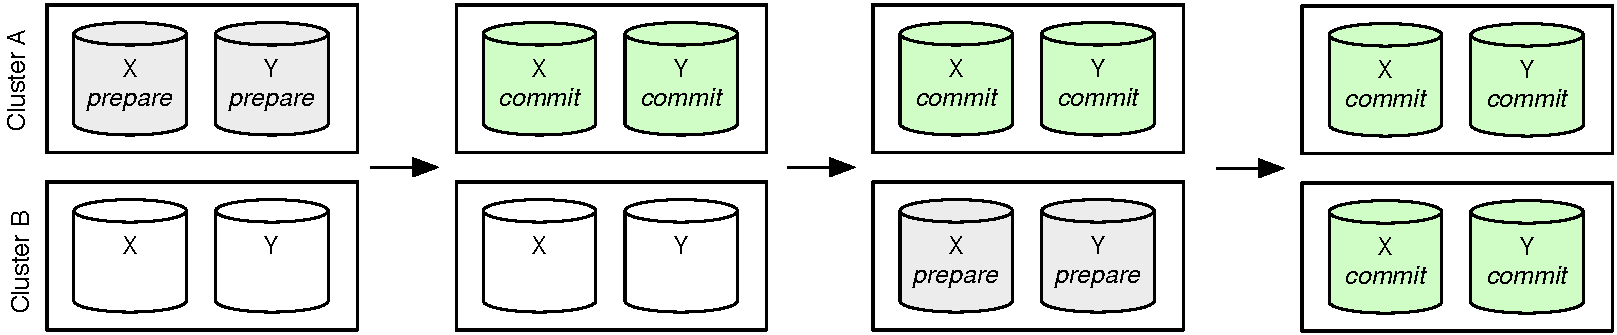
\includegraphics[width=\textwidth]{diagram/mdc-sticky.pdf}
\label{fig:mdc-sticky}
}\vspace{1em}

\caption{Control flow for operations under multi-datacenter RAMP strategies with client in Cluster A writing to partitions X and Y. In the high availability RAMP strategy (Figure~\ref{fig:mdc-ha}), a write must be prepared on $F+1$ servers (here, $F=3$) before is committed. In the sticky RAMP strategy, a write can be prepared and committed within a single datacenter and asynchronously propagated to other datacenters, where it is subsequently prepared and committed (Figure~\ref{fig:mdc-sticky}). The sticky strategy requires that clients maintain affinity with a single cluster in order to guarantee available and correctly isolated behavior.} 
 \end{center} \label{fig:mdc} \end{figure}


\minihead{\textit{Prepare-F HA RAMP}} The first strategy is easier to understand but perhaps less practical. A client specifies a minimum durability for its write operations, measured in terms of number of failures it wishes to survive, $F$. When writing, the client issues a prepare request to all clusters and waits until it receives a successful response from $F+1$ servers. This ensures that the client's write is durable, and the client knows its intent has been logged on at least $F+1$ servers. The client transaction subsequently returns success (Figure~\ref{fig:mdc-ha}). Once all servers have received the prepare request (which is detectable via either via server-server communication as in the CTP protocol or via an asynchronous callback on the client), the servers can begin to commit the client's writes autonomously. This preserves RA isolation---but at a cost. Namely, there is no guarantee of \textit{visibility} of writes: a client is not guaranteed to read its own writes. Moreover, if a single server is offline, the servers will not begin the commit step, and clients will not observe the effects of the prepared transactions for an indefinite period of time. By ensuring availability of writes (i.e., clients return early), we have sacrificed visibility in the form of ensuring that writes are accessible to readers. Thus, clients will not enjoy session guarantees~\cite{sessionguarantees} such as Read Your Writes. Given the importance of these session guarantees for many of the industrial users we have encountered (e.g., see Facebook's TAO geo-replication~\cite{tao}), we currently do not favor this approach.

\minihead{\textit{Sticky HA RAMP}} The second strategy is to ensure a degree of stickiness, or affinity, between clients and servers within a datacenter~\cite{hat-vldb}.  Each client is assigned its own datacenter.  Instead of having a client issue its writes to the entire database replica set, the client can instead issue its prepare and commit operations to its assigned datacenter (or local replica group) and subsequently forward the writes to be prepared and committed autonomously in separate clusters (Figure~\ref{fig:mdc-sticky}). That is, once a writer has performed the appropriate RAMP protocol in its assigned datacenter, it can return.  In an $N$-datacenter deployment, each full write protocol is performed $N$ separate times---once per datacenter. If the same timestamp is assigned to each write, the end state of each datacenter will be equivalent. As long as clients remain connected to the \textit{same} datacenter (i.e., is ``sticky'' with respect to its database connections), it will read its writes.

The total number of prepare and commit operations are the same as in the first strategy, but the commit point is staggered---each cluster reaches a commit point independently, at different times. Moreover, clusters operate independently, so throughput is not improved---only latency---because each cluster must replay every other cluster's writes~\cite{explicit-socc}. This is the basic strategy espoused by traditional log shipping approaches~\cite{lazyreplication} as well as more recent proposals such as the COPS~\cite{cops} and Eiger~\cite{eiger} systems.

However, this stickiness has an often-neglected penalty: a client can no longer connect to arbitrary servers and expect to read its own writes. If a server is down in a client's local datacenter, the client must---in the worst case---locate an entire other replica set to which the client can connect. This negatively affects availability: the \textit{Prepare-F} strategy can utilize all servers at once, but the sticky strategy requires clients to maintain affinity for availability. In cases when this ``sticky availability''~\cite{hat-vldb} is acceptable (e.g., each datacenter contains a set of application servers that issue the RAMP protocols against another datacenter-local set of storage servers), this may be a reasonable compromise.

\subsection{Quorum-Replicated RAMP Operation}
\label{sec:quorum}

 While RAMP \textit{Prepare-F} and \textit{Sticky HA} are best suited for multi-datacenter deployments, in quorum-replicated systems such as Dynamo and Cassandra~\cite{cassandra-sigmod,dynamo}, there are several optimizations that can be used to further improve availability, even within a single datacenter.

Our key observation here is that, to guarantee maximum of two-round trips for reads, only \textsc{prepare} and second-round \textsc{get} requests need to intersect on a given set of replicas. Recall that second-round \textsc{get} requests are issued in order to ``repair'' any fractured reads from the first round of read results. In the event of these fractured reads, a reader \textit{must} have access to versions corresponding to fractured reads that have been prepared but were not committed at the time of the first-round read. However, assembling the first round of committed versions can run under partial (i.e., non-intersecting) quorum operation~\cite{prob-quorum} with respect to commit messages.

This means that \textsc{commit} and first-round \textsc{get} operations can proceed on effectively any server in a set of replicas, enabling two key optimizations. In these optimizations, we assume that readers issue second-round read requests and writers issue \textsc{prepare} operations using a quorum system~\cite{naor-quorums} of replicas (e.g., majority quorums).

First, first-round read requests can be served from any replica of a given item. Then, if a client detects a race (in \rapl or \rapb), it can issue the optional second round of requests to a quorum of servers. \raps will always issue the second round of requests. This optimization improves the latency of the first round of reads and also enables speculative retry~\cite{tailscale}. It also decreases the load on the servers and increases availability for first-round read operations.

Second, commit operations can be performed on any replica of a given item. Similar to the optimization proposed in \textit{Prepare-F} RAMP, servers can propagate commit messages between themselves asynchronously, possibly piggybacking on anti-entropy messages as in systems like Cassandra and Dynamo. This optimization improves the latency of commit. However, because all servers must commit the transaction eventually, it does not necessarily decrease the load on servers.

To quantify the potential latency improvements achievable using these optimizations, we draw on latency distributions from a recent study of Dynamo-style operation~\cite{pbs-vldbj2013}. According to latency data from a Dynamo-style quorum-replicated database running on spinning disks at LinkedIn, moving from waiting for two replicas of three to respond to waiting for one replica of three to respond to a write request decreased latency from 21.0ms to 11.0ms at the 99.9th percentile; 1.63ms to 0.66ms for reads. For a similar database at Yammer, the gains for writes are 427ms to 10.8ms and the gains for reads are 32.6ms  to 5.6ms---an even more impressive gain. Over a wide-area network with latency of 75ms, the gains are as much as 148ms. Thus, in practice, these simple optimizations may prove worthwhile.

\subsection{RAMP, Transitive Dependencies, and Causal Consistency}
\label{sec:causal}

In Section~\ref{sec:ra-compare}, we discussed how RA isolation does not enforce transitive read-write dependencies across transactions. For example, if $T_a$ read-depends on $T_b$ (i.e., $T_a$ reads a version that $T_b$ created), another transaction $T_c$ might read-depend on $T_a$ (i.e., $T_c$ reads a version that $T_a$ created) but anti-depend on $T_b$ (i.e., $T_b$ overwrites a version that $T_a$ read). In this section, we discuss why we made this design decision as well as alternatives for enforcing dependencies and their costs.

% why did we do this?

The primary challenges in enforcing transitive dependencies come in limiting metadata while preserving availability and partition independence. In the extreme, if we limited ourselves to serial access to database state, we could easily preserve information about dependencies using a single scalar: any transactions would observe versions with lower scalar values, similar to classic serializable multi-version concurrency control. However, if we wish to preserve available and coordination-free operation (and therefore concurrent creation of versions), then we must admit a partial ordering of versions. To avoid fractured reads as in RA isolation while preserving dependency information, we either need to find a way to capture this partial order or otherwise limit the degree of availability in the system.

\minihead{Full causality tracking} The former approach---tracking ``cuts'' in a system with partially ordered events---is well-studied. As a first approximation, we can consider the problem of capturing RA with dependency tracking as an instance of capturing causality in a distributed system, with each event corresponding to a transaction commit and dependencies due to reads (i.e., a causal memory with atomically visible, multi-register reads). In line with this approximation, we could replace each timestamp in the RAMP algorithms with a suitable mechanism for tracking causality; for example, instead of storing a scalar timestamp, we could store a vector clock, with one entry per client in the system. Subsequently, clients could maintain a vector clock containing the highest-committed writes they had seen, and, upon reading from servers, ensure that the server commits any writes that happen-before the client's current vector. Thus, we can use vector clocks to track dependencies across transactions.

The problem with the above approach is in the size of the metadata required. Primarily, with $N$ concurrent clients, each vector will require $O(N)$ space, which is potentially prohibitive in practice. Moreover, the distributed systems literature strongly suggests that, with $N$ concurrent clients, $O(N)$ space is \textit{required} to capture full causal lineage as above~\cite{vc-lowerbound}. Thus, while using vector clocks to enforce transitive dependencies is a correct approach, it incurs considerable overheads that we do not wish to pay and have yet to be proven viable at scale in practical settings~\cite{explicit-socc}.\footnote{Another alternative that uses additional metadata is the strawman from Section~\ref{sec:sysmodel}, in which clients send all of the writes in their transaction to all of the partitions responsible for at least one write in the transaction. This uses even more metadata than the vector-based approach.}

The latter approach---limiting availability---is also viable, at the cost of undercutting our scalability goals from Section~\ref{sec:sysmodel}.

\minihead{Bounding writer concurrency} One simple approach---as we hinted above---is to limit the concurrency of writing clients: we can bound the overhead of vector clocks to an arbitrarily small amount by limiting the amount of concurrency in the system. For example, if we allow five clients to perform writes at a given time, we only need a vector of size five. This requires coordination between writers (but not readers). As Section~\ref{sec:eval-compare} demonstrated, RAMP transaction performance degrades gracefully under write contention; under the decreased concurrency strategy, performance would effectively hit a cliff. Latency would increase due to queuing delays and write contention, and, for a workload like YCSB with a fixed proportion of read to write operations, throughput would be limited. Specifically, for a workload with $p$ writers ($p=0.05$ in our default configuration), if $W$ writers were permitted at a given time, the effective number of active YCSB clients in the system would become $\frac{W}{p}$. Despite these limits, this is perhaps the most viable solution we have encountered and, moreover, does not affect read performance under read-heavy workloads. However, this solution has considerable coordination overheads, and managing which servers are able to perform writes (e.g., using distributed leases) requires potentially heavyweight synchronization protocols.

\minihead{Sacrificing partition independence} Another approach to improving availability is to sacrifice partition independence. As we discuss and evaluate in Sections~\ref{sec:setup} and~\ref{sec:eval-compare}, it is possible to preserve transaction dependencies by electing special coordinator servers as points of rendezvous for concurrently executing transactions. If extended to a non-partition-independent context, the RAMP protocols begin to more closely resemble traditional multi-version concurrency control solutions, in particular, Chan and Gray's read-only transactions~\cite{readonly}. More recently, the 2PC-PCI mechanism~\cite{eiger} we evaluated is an elegant means of achieving this behavior if partition independence is unimportant. Nevertheless, as our experimental evaluation shows, sacrificing this partition independence can be costly under some workloads.

\minihead{Sacrificing causality} A final approach to limiting the overhead of dependency tracking is to limit the number of dependencies to track. Several prior systems have used limited forms of causality, for example, application-supplied dependency information~\cite{bolton,lazyreplication}, as a basis for dependency tracking. In this strategy, applications inform the system about what versions should precede a given write; in~\cite{explicit-socc} (see also Section~\ref{sec:explicitcausality}), we show that, for many modern web applications, these histories can be rather small (often one item, with a power-law distribution over sizes). In this case, we could encode the causal history in its entirety along with each write or exploit otherwise latent information within the data such as comment \texttt{reply-to} fields to mine this data automatically. This strategy breaks the current RAMP API. However, it is the only known strategy for circumventing the $O(N)$ upper-bound on dependency tracking in causally consistent storage systems ensuring availability of both readers and writers.

\minihead{Experiences with system operators} While causal consistency provides a number of useful guarantees, in practice, we perceive a lack of interest in maintaining full causal consistency; database operators and users are anecdotally often unwilling to pay the metadata and implementation costs of full causality tracking. As we have seen in Section~\ref{sec:motivation}, many of these real-world operators exhibit an aversion to synchronization at scale, so maintaining availability is paramount to either their software offerings or business operation. In fact, we have anecdotally found coordination-free execution and partition independence to be valuable selling points for the RAMP algorithms presented in this work. Instead, we have found many users instead favor guarantees such as Read Your Writes (provided by the RAMP algorithms) rather than full dependency tracking, opting for variants of explicit causality (e.g., via foreign key constraints or explicit dependencies) or restricted, per-item causality tracking (e.g., version vectors~\cite{dynamo}). Despite this mild pessimism, we view further reduction of causality overhead to be an interesting area for future work---including a more conclusive answer to the availability-metadata trade-off surfaced by~\cite{vc-lowerbound}.


\FloatBarrier

\begin{comment}
\subsection{In Detail: Index Maintenance with RAMP}
\label{sec:index-detail}

In this section, we present additional detail about index maintenance with RAMP transactions. In our presentation of the RAMP thus far, we have largely concerned ourselves with opaque reads and writes to items defined by the user. In contrast, the writes required to perform index maintenance are \textit{not} opaque to the system and are well-defined (and often repetitive; e.g., of the form: ``update the index entry for value \textit{v} by adding ID \textit{i}''). Thus, in the case of index maintenance, we can exploit the structure of the data (as hinted in Section~\ref{sec:causal} to improve algorithm efficiency. We present details in two stages: performing insertions and updates, and issuing queries.

\minihead{Performing Insertions and Updates} When a base table is modified, the database system can automatically generate the appropriate set of updates to corresponding index entries to be applied as part of a RAMP write transaction upon transaction commit. If we represent indexes as a mapping from values (e.g., hair color) to a set of matching items (e.g., item and version), insertions generate an addition to a set, and deletions generate a deletion from a set.



\minihead{Issuing Queries}
\end{comment}



\chapter{Related Work}
\label{c.relatedwork}

In this chapter, we provide a discussion of related work. We begin
with a discussion of work related to the general themes in this
thesis, then examine specific areas in depth.


Database system designers have long sought to manage the trade-off
between consistency and coordination. As we have discussed,
serializability and its many implementations (including lock-based,
optimistic, and pre-scheduling
mechanisms)~\cite{silo,bernstein-book,tamer-book,hstore,gray-virtues,calvin,eswaran-consistency,sdd1}
are sufficient for maintaining application correctness. However,
serializability is not always necessary: serializable databases do not allow certain
executions that are correct according to application semantics.  This
has led to a large class of application-level---or
semantic---concurrency control models and mechanisms that admit
greater concurrency. There are several surveys on this topic, such
as~\cite{tamer-book,ic-survey}, and, in our solutions, we integrate
many concepts from this literature.

\minihead{Commutativity} One of the most popular alternatives to
serializability is to exploit \textit{commutativity}: if transaction
return values (e.g., of reads) and/or final database states are
equivalent despite reordering, they can be executed
simultaneously~\cite{weihl-thesis,kohler-commutativity,redblue}. Commutativity
is often sufficient for correctness but is not necessary. For example,
if an analyst at a wholesaler creates a report on daily cash flows,
any concurrent sale transactions will \textit{not} commute with the
report (the results will change depending on whether the sale
completes before or after the analyst runs her queries). However, the
report creation is \iconfluent with respect to, say, the invariant
that every sale in the report references a customer from the customers
table. \cite{kohler-commutativity,lamport-audit} provide additional
examples of safe non-commutativity.

\minihead{The CALM Theorem, Monotonicity, and Confluence}
Hellerstein's CALM Theorem~\cite{ameloot-calm} shows that program
outcomes are confluent, or deterministic, under coordination-free
execution if and only if the program logic is monotone. CALM is a
declarative result: it captures the class of computations that can be
implemented deterministically without coordination. CALM can also be
used as a program analysis technique: if a particular program
implementation uses only monotonic operations (where ``program'' could
include a service and its client code), then that program will be
deterministic when executed without coordination; otherwise,
coordination should be injected to ``protect'' non-monotonic
operations to ensure determinism.  CALM program analysis is natural to
apply in logic languages like Bloom~\cite{calm} where monotonicity can
be assessed from syntax.  It can also be applied to dataflow systems
like Storm~\cite{storm} with the help of program
annotations~\cite{blazes}.

CALM's notion of confluence differs from invariant confluence in
several ways. First, CALM assesses the confluence, or determinism, of
program logic; invariant confluence assesses whether a set of safety
properties holds during and following the execution of a set of
transactions over replicated or multi-versioned data given a
particular merge function. \Iconfluence admits non-deterministic
outcomes as long as the outcomes satisfy the provided invariants.
Second, CALM does not consider transactions, while invariant
confluence analyzes transactions that individually ensure
invariant-preserving updates.  Third, invariant confluence considers
replicated or multi-versioned state (via the use of the replica
abstraction). As discussed in Section~\ref{sec:model}, invariant
confluent does not distinguish between partially-replicated and
fully-replicated systems; under invariant confluence, a transaction is
presented with an entire logical snapshot (replica) of the database
upon which it can operate. A partially replicated implementation of a
set of \iconfluent operations may need to communicate with partitions
responsible for items that were not explicitly mentioned in the
transaction operations but that are related to invariants over data
modified by the transaction. Again, and by
Theorem~\ref{theorem:necessary}, for \iconfluent semantics, this
checking can be performed in parallel by concurrently committing
transactions over their respective logical replicas. However, in
contrast, CALM analysis is agnostic to replication, versioning, and
partitioning, which, if desired, are implemented as part of program
logic to be analyzed.

CALM and invariant confluence use different mathematical
foundations. CALM is based on monotonicity analysis from logic
programs. \Iconfluence generalizes classic partitioning arguments from
distributed systems to the domain of user-supplied invariants,
transactions, and merge functions. For associative, commutative, and
idempotent merge functions, an \iconfluent execution effectively
defines a join semi-lattice: invariants begin true in $D_0$ and remain
true as the execution progresses. Monotone programs also compute over
a join semi-lattice of relations and union. However, the analyses and
proof techniques of the two concepts are quite different.

Further understanding the relationship between invariant confluence
and CALM is an interesting area for exploration. For example, it is
natural to ask if there is an extension of CALM analysis that can,
like \iconfluence, incorporate invariants over possibly
non-deterministic outputs. A possible direction here is to view
invariants as boolean-valued formulas whose results ``start true'' and
monotonically remain true. In this direction, an invariant is a
morphism mapping from potentially monotone relational inputs to a
monotone boolean output lattice~\cite{blooml}.  Additionally, as CALM
is non-transactional and our formulation of invariant confluence is
inherently transactional, it is interesting to consider what
``transactional CALM'' would mean. In our formulation of \iconfluence,
transactions that violate invariants when committing to local replica
state are aborted; it is unclear how to model abort logic in CALM
analysis.

\minihead{Convergent Data Types} On a related subject, Commutative
Replicated Data Type (CRDT) objects~\cite{crdt} similarly ensure
convergent outcomes that reflect all updates made to each object.
This convergence is a useful \textit{liveness}
property~\cite{schneider-concurrent} (e.g., a converged CRDT OR-Set
reflects all concurrent additions and removals) but does not prevent
users from observing inconsistent data~\cite{redblue-new}, or
\textit{safety} (e.g., the CRDT OR-Set does not---by itself---enforce
invariants, such as ensuring that no employee belongs to two
departments), and are therefore not sufficient to guarantee
correctness for all applications. Here, we use CRDTs to implement many
of our merge functions, and we add safety to the intermediate states
and final outcomes. Thus, each replica state is, in effect, a CRDT,
and our goal is to determine which operations need coordination to
ensure variants of safety properties are upheld.

\minihead{Use of Invariants} A large number of database
designs---including, in restricted forms, many commercial databases
today---use various forms of application-supplied invariants,
constraints, or other semantic descriptions of valid database states
as a specification for application correctness
(e.g.,~\cite{korth-serializability,kemme-si-ic,garciamolina-semantics,ic-survey,ic-survey-two,decomp-semantics,redblue,homeostasis,davidson-survey,local-verification,redblue-new,rel-serial,pwsr-pods,tamer-tods}). We
draw inspiration and, in particular, our use of invariants from this
prior work. However, we are not aware of related work that discusses
when coordination is strictly \textit{required} to enforce a given set
of invariants. That is, our formulation of coordination-free execution
of transactions on separate replicas, which is key to capturing
scalability, low latency, and availability properties, is not found in
this related work; we, in effect, operate at the junction between this
prior work on semantics-based concurrency control from databases and
classic analyses from distributed
computing~\cite{gilbert-cap}. 

To illustrate why replication is so important to our model, consider
the work on relative serializability~\cite{rel-serial}. In this work,
the authors generalize prior efforts,
including~\cite{korth-serializability,garciamolina-semantics,atomictransactions,tamer-tods},
and re-define conflicting actions within otherwise conflict
serializable transaction execution in order to allow greater
concurrency. That is, instead of defining conflict as ``any two
operations on the same item from different transactions, at least one
of which is a write'' as in conflict serializability, relative
serializability allows users to define an abstract atomicity relation
to determine conflicts---for example, two increment operations need
not necessarily conflict, even if they both update the same
counter. Thus, the goal of this work is to preserve equivalence a
serial schedule, defined according to the abstract atomicity relation,
and there is still a total order on operations. As a result, in
relative serializability and related models~\cite{pwsr-pods}, the
``union'' (or combination) of two databases is undefined if two items
have different versions (e.g., $\{a_1\} \cup \{a_2\}$), because such
databases would correspond to two separate total orders. In contrast,
in our \iconfluence analysis, we explicitly consider a partial order
on operations, with divergent states reconciled with a merge operator;
instead of reasoning about conflicts, we allow arbitrary divergent
states that $i)$ are guaranteed to satisfy a user-specified invariant
over the data and $ii)$ are reconciled using a user-specified merge
function.

Because data is replicated in our model, it is natural to reason about
a ``merge'' function. Insofar as servers must explicitly integrate
updates from others in order to guarantee convergence (in contrast
with conventional shared-memory systems, where hardware automatically
chooses an ordering and conflict resolution policies for updates),
merge allows users to specify their own conflict resolution. As we
have discussed, the merge operator is itself drawn from the literature
on optimistic replication~\cite{optimistic} and is relatively popular
today in stores including Dynamo~\cite{dynamo} and its descendants as
well as systems like Git. Thus, while the goals of work on
semantics-based concurrency control (including relative
serializability) are similar to ours (especially in terms of
increasing concurrency), our use of merge leads to a substantially
different system and execution model. In effect, we can think of
\iconfluence as relative serializability with a special,
system-induced compensating action (``merge'') to deal with divergent
paths in the semantic serializability serialization graph (RSG), if
the graph were extended to account for replication.

Thus, our \iconfluence analysis here is inspired by prior work on
semantics-based concurrency control and adapts the practice of using
application (and database) criteria as the basis of concurrency
control to the replicated (and non-serializable, multi-versioned)
setting. Moreover, compared to this prior work, our practical focus
here is oriented towards invariants found in SQL and in modern
applications.

In contrast with many of the conditions above (esp. commutativity and
monotonicity), we explicitly require more information from the
application in the form of invariants (Kung and
Papadimitriou~\cite{kung1979optimality} suggest this is information is
\textit{required} for general-purpose non-serializable yet safe
execution.)  In this work, we provide a necessary and sufficient
condition for safe, coordination-free execution over replicated and
multi-version data. When invariants are unavailable, many of these
more conservative approaches may still be applicable. Our use of
analysis-as-design-tool is inspired by this literature---in
particular,~\cite{kohler-commutativity}.


\minihead{Coordination costs} In this work, we determine when
transactions can run entirely concurrently and without
coordination. In contrast, a large number of alternative models
(e.g.,~\cite{garciamolina-semantics,korth-serializability,isolation-semantics,local-verification,kemme-si-ic,aiken-confluence,laws-order})
assume serializable or linearizable (and therefore coordinated)
updates to shared state. These assumptions are standard (but not
universal~\cite{ec-txns}) in the concurrent programming
literature~\cite{schneider-concurrent,laws-order}. (Additionally,
unlike much of this literature, we only consider a single set of
invariants per database rather than per-operation invariants.) For
example, transaction chopping~\cite{chopping} and later
application-aware
extensions~\cite{decomp-semantics,agarwal-consistency} decompose
transactions into a set of smaller transactions, providing increased
concurrency, but in turn require that individual transactions execute
in a serializable (or strict serializable) manner.  This reliance on
coordinated updates is at odds with our goal of coordination-free
execution. However, these alternative techniques are useful in
reducing the duration and distribution of coordination once it is
established that coordination is required.

\minihead{Term rewriting} In term rewriting systems, \iconfluence
guarantees that arbitrary rule application will not violate a given
invariant~\cite{obs-confluence}, generalizing Church-Rosser
confluence~\cite{termrewriting}. We adapt this concept and effectively
treat transactions as rewrite rules, database states as constraint
states, and the database merge operator as a special \textit{join}
operator (in the term-rewriting sense) defined for all
states. Rewriting system concepts---including
confluence~\cite{aiken-confluence}---have previously been integrated
into active database systems~\cite{activedb-book} (e.g., in triggers,
rule processing), but we are not familiar with a concept analogous to
\iconfluence in the existing database literature.

\minihead{Coordination-free algorithms and semantics} Our work is
influenced by the distributed systems literature, where
coordination-free execution across replicas of a given data item has
been captured as ``availability''~\cite{gilbert-cap,queue}. A large
class of systems provides availability via ``optimistic replication''
(i.e., perform operations locally, then
replicate)~\cite{optimistic}. We---like others~\cite{ec-txns}---adopt
the use of the merge operator to reconcile divergent database
states~\cite{bayou} from this literature. Both traditional database
systems~\cite{adya} and more recent
proposals~\cite{redblue-new, redblue} allow the simultaneous use of
``weak'' and ``strong'' isolation; we seek to understand \textit{when}
strong mechanisms are needed rather than an optimal implementation of
either. Unlike ``tentative update'' models~\cite{sagas}, we do not
require programmers to specify compensatory actions (beyond merge,
which we expect to typically be generic and/or system-supplied) and do
not reverse transaction commit decisions. Compensatory actions could
be captured under \iconfluence as a specialized merge procedure.

The CAP Theorem~\cite{gilbert-cap,pacelc} recently popularized the
tension between strong semantics and coordination and pertains to a
specific model (linearizability). In a recent retrospective, Brewer
discusses the role of CAP in reasoning about and ``repairing'' more
general invariants, such as those we study
here~\cite{brewer-cap}. The relationship between serializability and
coordination requirements has also been well documented in the
database literature~\cite{davidson-survey}. Our research here
addresses when particular database-backed applications require
coordination, providing a new property, \iconfluence, for doing so.

\minihead{Summary} The \iconfluence property is a necessary and
sufficient condition for safe, coordination-free execution. Sufficient
conditions such as commutativity and monotonicity are useful in
reducing coordination overheads but are not always necessary. Here, we
explore the fundamental limits of coordination-free execution. To do
so, we explicitly consider a model without synchronous
communication. This is key to scalability: if, by default, operations
must contact a centralized validation service, perform atomic updates
to shared state, or otherwise communicate, then scalability will be
compromised. Finally, we only consider a single set of invariants for
the entire application, reducing programmer overhead without affecting
our \iconfluence results.



\subsubsection{Isolation and RAMP Transactions}

Replicated databases offer a broad spectrum of isolation guarantees at
varying costs to performance and availability~\cite{bernstein-book}:

\minihead{Serializability} At the strong end of the isolation spectrum
is serializability, which provides transactions with the equivalent of
a serial execution (and therefore also provides RA). A range of
techniques can enforce serializability in distributed
databases~\cite{bernstein-book,divy-writeonly}, multi-version
concurrency control (e.g.~\cite{mv-mobile}), locking
(e.g.~\cite{versions-update}), and optimistic concurrency
control~\cite{f1}. These useful semantics come with costs in the form
of decreased concurrency (e.g., contention and/or failed optimistic
operations) and limited availability during partial
failure~\cite{hat-vldb,davidson-survey}. Many
designs~\cite{hstore,gstore} exploit cheap serializability within a
single partition but face scalability challenges for distributed
operations. Recent industrial efforts like F1~\cite{f1} and
Spanner~\cite{spanner} have improved performance via aggressive
hardware advances but, their reported throughput is still limited to
20 and 250 writes per item per second. Multi-partition,
multi-datacenter, and, generally, distributed serializable
transactions are expensive and, especially under adverse conditions,
are likely to remain
expensive~\cite{schism,jones-dtxn,pavlo-partition}.

\minihead{Weak isolation} The remainder of the isolation spectrum is
more varied. Most real-world databases offer (and often default to)
non-serializable isolation models~\cite{mohan-note,hat-vldb}. These
``weak isolation'' levels allow greater concurrency and fewer
system-induced aborts compared to serializable execution but provide
weaker semantic guarantees. For example, the popular choice of
Snapshot Isolation prevents Lost Update anomalies but not Write Skew
anomalies~\cite{adya}; by preventing Lost Update,
concurrency control mechanisms providing Snapshot Isolation require coordination~\cite{hat-vldb}. In recent years, many
``NoSQL'' designs have avoided cross-partition transactions entirely,
effectively providing Read Uncommitted isolation in many industrial
databases such PNUTS~\cite{pnuts}, Dynamo~\cite{dynamo},
TAO~\cite{tao}, Espresso~\cite{espresso}, Rainbird~\cite{rainbird},
and BigTable~\cite{bigtable}. These systems avoid penalties associated
with stronger isolation but in turn sacrifice transactional guarantees
(and therefore do not offer RA).

%Swift~\cite{swift}, 

\minihead{RAMP and related mechanisms} There are several algorithms that are
closely related to our choice of RA and RAMP algorithm design.

COPS-GT's two-round read-only transaction protocol~\cite{cops} is
similar to \rapl reads---client read transactions identify causally
inconsistent versions by timestamp and fetch them from servers. While
COPS-GT provides causal consistency (requiring additional metadata),
it does not support RA isolation for multi-item writes.

Eiger provides its write-only transactions~\cite{eiger} by electing a
coordinator server for each write. As discussed in
Section~\ref{sec:ramp-evaluation} (\mstr), the number of ``commit checks''
performed during its read-only transactions is proportional to the
number of concurrent writes. Using a coordinator violates partition
independence but in turn provides causal consistency. This coordinator
election is analogous to G-Store's dynamic key grouping~\cite{gstore}
but with weaker isolation guarantees; each coordinator effectively
contains a partitioned completed transaction list
from~\cite{readonly}. Instead of relying on indirection, RAMP
transaction clients autonomously assemble reads and only require
constant factor (or, for \rapl, linear in transaction size) metadata
size compared to Eiger's \textit{PL-2L} (worst-case linear in database
size).

We are not aware of another concurrency control mechanism for
partitioned databases that ensures coordination-free execution,
partition independence, and at least RA isolation.

\subsubsection{Constraints}

There is a large body of related work related to our investigation of
specific database and ORM constraints that we consider in three
categories: object relational mapping systems, the quantification of
isolation behavior, and empirical open source software analysis.

\minihead{ORMs} Database systems and application programming
frameworks have a long
history~\cite{objectstore,shore,bernstein-orm}. The ``impedance
mismatch'' between object-oriented programming and the relational
model is a perennial problem in data management systems. Ruby on Rails
is no exception, and the concurrency control issues we study here are
endemic to this mismatch---namely, the disuse of common concurrency
control mechanisms like database-backed constraints. Bridging this gap
remains an active area of research~\cite{db-to-model}.

The latest wave of web programming frameworks has inspired diverse
research spanning databases, verification, and security. StatusQuo
uses program analysis and synthesis to transform imperative ORM code
into SQL, leveraging the efficiency of database-backed web
applications written in the Spring framework~\cite{statusquo}. Rails
has been the subject of study in the verification of cross-site
scripting attacks~\cite{rails-xss}, errors in data
modeling of associations~\cite{rails-bounded}, and arbitrary,
user-specified (non-validation) invariants~\cite{invariant-web}.
Rails-style ORM validations have been used to improve systems security
via client-side execution~\cite{waves,caveat}. Our focus here is on
the concurrency control requirements and usages of applications
written in Rails.

\minihead{Quantifying anomalies} A range of research similarly
quantifies the effect of non-serializable isolation in a variety of
ways.

Perhaps closest to our examination of ORM integrity violations is a
study by Fekete et al., which quantitatively analyzed data
inconsistencies arising from non-serializable
schedules~\cite{fekete-quantifying}. This study used a hand-crafted
benchmark for analysis but is nevertheless one of the only studies of
actual application inconsistencies. Here, we focus on open source
applications from the Rails community.

A larger body of work examines isolation anomalies at the read-write
interface (that is, measures deviations from properties such as
serializability or linearizability but \textit{not} the end effect of
these deviations on actual application behavior). Wada et
al. evaluated the staleness of Amazon's SimpleDB using end-user
request tracing~\cite{wada-data}, while Bermbach and Tai evaluated
Amazon S3~\cite{bermbach-eventual}, each quantifying various forms of
non-serializable behavior. Golab et al. provide algorithms for
verifying the linearizability of and sequential consistency arbitrary
data stores~\cite{golab-analyzing} and Zellag and Kemme provide
algorithms for verifying their
serializability~\cite{zellag-consistent} and other cycle-based
isolation anomalies~\cite{zellag-real}. As we have discussed,
Probabilistically Bounded Staleness provides time- and version-based
staleness predictions for eventually consistent data
stores~\cite{pbs}. Our focus here is on anomalies as observed by
application logic rather than read-write anomalies observed under weak
isolation.

\minihead{Empirical software analysis} Empirical software analysis of
open source software is a topic of active interest in the software
engineering research community~\cite{foss-icse}. In the parlance of
that community, in this work, we perform a mixed-methods analysis,
combining quantitative survey techniques with a confirmatory case
study of Rails's susceptibility to validation
errors~\cite{empiricalmethods}. In our survey, we attempt to minimize
sampling bias towards validation-heavy projects by focusing our
attention on popular projects, as measured by GitHub stars. Our use of
quantitative data followed by supporting qualitative data from
documentation and issue tracking---as well as the chronology of
methodologies we employed to attain the results presented here---can
be considered an instance of the sequential exploration
strategy~\cite{creswell2013research}. We specifically use these techniques in
service of better understanding use of database
concurrency control.



\newcommand{\transform}{\textsc{Transform}\xspace}

\section{RSIW Proof}

\label{sec:rsiwproof}


% total order valid because G1c is prohibited

To begin, we first show that there exists a well-defined total
ordering of write-only transactions in a history that is valid under
RA isolation. This will be useful in ordering write transactions in
our one-copy equivalent execution.

\begin{lemma}[Well-defined Total Order on Writes]
\label{lemma:to}
  Given a history $H$ containing read-only and write-only transactions
  that is valid under RA isolation, $DSG(H)$ does not contain any
  directed cycles consisting entirely of write-dependency edges.
\end{lemma}
\begin{proof}
  $H$ is valid under RA isolation and therefore does not exhibit
  phenomenon \textit{G1c}. Thus, $H$ does not contain any directed
  cycles consisting entirely of dependency edges. Therefore, $H$ does
  not contain any directed cycles consisting entirely of
  write-dependency edges.
\end{proof}

We will also need to place read-only transactions in our history. To
do so, we show that, under RA isolation and the RSIW property (i.e.,
the preconditions of Theorem~\ref{thm:rsw}), each read-only
transaction will only read from one write-only transaction.

\begin{lemma}[Single Read Dependency]
\label{lemma:onedep}
Given a history $H$ containing read-only and write-only transactions
that obeys the RSIW property and is valid under RA isolation, each
node in $DSG(H)$ contains at most one direct read-dependency edge.
\end{lemma}
\begin{proof}
  Consider a history $H$ containing read-only and write-only
  transactions that has RSIW and is valid under RA
  isolation. Write-only transactions have no reads, so they have no
  read-dependency edges in $DSG(H)$. However, suppose $DSG(H)$
  contained a node corresponding to a read-only transaction containing
  more than one direct read-dependency edge; call this read-only
  transaction $T_r$. For two read-dependency edges to exist, $T_r$
  must have read versions produced by at least two different
  write-only transactions; pick any two and call them $T_i$ and $T_j$,
  corresponding to read versions $x_a$ and $y_d$.

  If $x$ and $y$ are the same item, then $a < d$ or $d < a$. In either
  case, $T_r$ exhibits the fractured reads phenomenon and $H$ is not
  valid under RA isolation, a contradiction.

  Therefore, $x$ and $y$ must be distinct items. Because $H$ obeys the
  RSIW property, $T_r$ must also obey the RSIW property. By the
  definition of the RSIW property, $T_r$ must have only read items
  written to by $T_i$ and items also written to by $T_j$; this implies
  that $T_i$ and $T_j$ each wrote to items $x$ and $y$. We can label
  $T_i$'s write to $y$ as $y_b$ and $T_j$'s write to $x$ as $x_c$. Per
  Lemma~\ref{lemma:to}, $T_i$'s writes to $x$ and $y$ must either both
  come before or both follow $T_j$'s corresponding writes to $x$ and
  $y$ in the version order for each of $x$ and $y$; that is, either
  both $a < b$ and $c < d$ or both $b < a$ and $d < c$.

  If $a < b$ and $c < d$, then $T_r$ exhibits the fractured reads
  phenomenon: $T_r$ read $x_a$ and $y_d$ but $T_j$, which wrote $y_d$
  also wrote $x_b$, and $a < b$. If $b < a$ and $d < c$, then $T_r$
  again exhibits the fractured reads phenomenon: $T_r$ read $x_a$ and
  $y_d$ but $T_i$, which wrote $x_a$, also wrote $y_c$, and $d <
  c$. In either case, $H$ is not valid under RA isolation, a
  contradiction.

  Therefore, each node in $DSG(H)$ must not contain more than one
  read-dependency edge.
\end{proof}

We now use this ordering on reads and writes to construct a total
ordering on transactions in a history:

\begin{procedure}[Transform]
  Given a history $H$ containing read-only and write-only transactions
  that has RSIW and is valid under RA isolation,
  construct a total ordering $O$ of the transactions in $H$ as
  follows:
\begin{enumerate}
\item Perform a topological sorting in $O$ of committed write-only
  transactions in $H$ ordered by the write-dependency edges in
  $DSG(H)$. That is, for each pair of write-only transactions ($T_1$,
  $T_2$) in $H$ that performed at least one write to the same item,
  place the transaction that wrote the higher-versioned item later in
  $O$. Lemma~\ref{lemma:to} ensures such a total ordering exists.
\item For each committed read-only transaction $T_r$ in $H$, place
  $T_r$ in $O$ after the write-only transaction $T_w$ whose writes
  $T_r$ read (i.e., after the write-only transaction that $T_r$
  directly read-depends on) but before the next write-only transaction
  $T_{w'}$ in $O$ (or, if no such transaction exists, at the end of
  $O$). By Lemma~\ref{lemma:onedep}, each committed read-only
  transaction read-depends on only one write-only transaction, so this
  ordering is similarly well defined.
\end{enumerate}

Return $O$.

\end{procedure}

As an example, consider the following history:
\begin{eqnarray}
\label{hist:transform-example}
T_1 & w(x_1); w(y_1)\\
T_2 & w(x_2); w(y_2)\nonumber\\
T_3 & r(x_1); r(y_1)\nonumber\\
T_4 & r(y_2);\nonumber
\end{eqnarray}
History~\ref{hist:transform-example} obeys the RSIW property and is
also valid under RA isolation. Applying procedure~\transform to
History~\ref{hist:transform-example}, in the first step, we first
order our write-only transactions $T_1$ and $T_2$. Both $T_1$ and
$T_2$ write to $x$ and $y$, but $T_2$'s writes have a later version
number than $T_1$'s, so, according to Step 1 of~\transform, we have
$O=T_1; T_2$. Now, in Step 2 of~\transform, we consider the read-only
transactions $T_3$ and $T_4$. We place $T_3$ after the transaction
that it read from ($T_1$) and before the next write transaction in the
sequence ($T_2$), yielding $O=T_1; T_3; T_2$. We place $T_4$ after the
transaction that it read from ($T_2$) and, because there is no later
write-only transaction following $T_2$ in $O$, place $T_4$ at the end
of $O$, yielding $O=T_1; T_3; T_2; T_4$. In this case, we observe
that, as Theorem~\ref{thm:rsw} suggests, it is possible to~\transform
an RSIW and RA history into a one-copy serial equivalent and that $O$ is in fact
a one-copy serializable execution.

Now we can prove Theorem~\ref{thm:rsw}. We demonstrate that executing
the transactions of $H$ in the order resulting from
applying~\transform to $H$ on a single-copy database yields an
equivalent history (i.e., read values and final database state) as
$H$. Because $O$ is a total order, $H$ must be one-copy serializable.
\begin{proof}[Theorem~\ref{thm:rsw}]
  Consider history $H$ containing read-only and write-only
  transactions that has RSIW and is valid under RA
  isolation. We begin by applying~\transform to $H$ to produce an
  ordering $O$. 

  We create a new history $H_o$ by considering an empty one-copy
  database and examining each transaction $T_h$ in $O$ in serial order
  as follows: if $T_h$ is a write-only transaction, execute a new
  transaction $T_{ow}$ that writes each version produced by $T_h$ to
  the one-copy database and commits. If $T_h$ is a read-only
  transaction, execute a new transaction $T_{or}$ that reads from the
  sam items as $T_h$ and commits. $H_o$ is the result of a serial
  execution of transactions over a single logical copy of the
  database, $H_o$ is one-copy serializable.

  We now show that $H$ and $H_o$ are equivalent. First, all committed
  transactions and operations in $H$ also appear in $H_o$
  because~\transform operates on all transactions in $H$ and all
  transactions and their operations (with single-copy operations
  substituted for multi-version operations) appear in the total order
  $O$ used to produce $H_o$. Second, $DSG(H)$ and $DSG(H_o)$ have the
  same direct read dependencies. This is a straightforward consequence
  of Step 2 of~\transform: in $O$, each read-only transaction $T_r$
  appears immediately following the write-only transaction $T_w$ upon
  which $T_r$ read-depends. When the corresponding read transaction is
  executed against the single-copy database in $H_o$, the serially
  preceding write-only transaction will produce the same values that
  the read transaction read in $H$. Therefore, $H$ and $H_o$ are equivalent.

  Because $H_o$ is one-copy serializable and $H_o$ is equivalent to $H$, $H$
  must also be one-copy serializable.
\end{proof}

We have opted for the above proof technique because we believe
the~\transform procedure provides clarity into \textit{how} executions
satisfying both RA isolation and the RSIW property relate to their
serializable counterparts. An alternative and elegant proof approach
leverages the work on multi-version serializability
theory~\cite{bernstein-book}, which we sketch here. Given a
history $H$ that exhibits RA isolation and has RSIW, we show
that $MVSG(H)$ is acyclic. By an argument resembling
Lemma~\ref{lemma:onedep}, the in-degree for read-only transactions in
$SG(H)$ (i.e., Adya's direct read dependencies) is one. By an argument
resembling Lemma~\ref{lemma:to}, the edges between write-only
transactions in $MVSG(H)$ produced by the first condition of the
$MVSG$ construction ($x_i \ll x_j$ in the definition of the
$MVSG$~\cite[p. 152]{bernstein-book}; i.e., Adya's write dependencies)
are acyclic. Therefore, any cycles in the $MVSG$ must include at least
one of the second kind of edges in the $MVSG(H)$ ($x_j \ll x_i$; i.e.,
Adya's direct anti-dependencies). But, for such a cycle to exist, a
read-only transaction $T_r$ must anti-depend on a write-only
transaction $T_{wi}$ that in turn write-depends on another write-only
transaction $T_{wj}$ upon which $T_r$ read-depends. Under the RSIW
property, $T_{wi}$ and $T_{wj}$ will have written to at least one of
the same items, and the presence of a write-dependency cycle will
indicate a fractured reads anomaly in $T_r$.

\section{RAMP Correctness and Independence}

\label{sec:rampproofs}


\minihead{RAMP-F Correctness} To prove \rapl provides RA isolation, we
show that the two-round read protocol returns a transactionally atomic
set of versions. To do so, we formalize criteria for atomic (read)
sets of versions in the form of \textit{companion sets}. We will call
the set of versions produced by a transaction \textit{sibling
  versions} and say that $x$ is a sibling item to a write $y_j$ if
there exists a version $x_k$ that was written in the same transaction
as $y_j$.

Given two versions $x_i$ and $y_j$, we say that $x_i$ is a
\textit{companion version} to $y_j$ if $x_i$ is a transactional
sibling of $y_j$ or $x$ is a sibling item of $y_j$ and $i > j$. We say
that a set of versions $V$ is a \textit{companion set} if, for every
pair $(x_i, y_j)$ of versions in $V$ where $x$ is a sibling item of
$y_j$, $x_i$ is a companion to $y_j$. In
Figure~\ref{fig:rapl-execution}, the versions returned by $T_2$'s
first round of reads ($\{x_1, y_\bot\}$) do not comprise a companion
set because $y_\bot$ has a lower timestamp than $x_1$'s sibling
version of $y$ (that is, $x_1$ has sibling version $y_1$ and but $\bot
< 1$ so $y_\bot$ has too low of a timestamp). Subsets of companion
sets are also companion sets and companion sets also have a useful
property for RA isolation:
\begin{claim}[Companion sets are atomic]
\label{claim:companion-atomic}
In the absence of G1c phenomena, companion sets do not contain fractured reads.
\end{claim}

Claim~\ref{claim:companion-atomic} follows from the definitions of
companion sets and fractured reads.

\begin{proof}
If $V$ is a companion set, then
every version $x_i \in V$ is a companion to every other version
$y_j \in V$ where $v_j$ contains $x$ in its sibling items. If $V$
contained fractured reads, $V$ would contain two versions $x_i,y_j$
such that the transaction that wrote $y_j$ also wrote a version $x_k$,
$i<k$. However, in this case, $x_i$ would not be a companion to
$y_j$, a contradiction. Therefore, $V$ cannot contain fractured reads.
\end{proof}

To provide RA, \rapl clients assemble a companion set for the
requested items (in $v_{latest}$), which we prove below:

\begin{claim}\rapl provides Read Atomic isolation.\end{claim}

\begin{proof}
\label{proof:rapl-ra}
Each write in \rapl contains information regarding its siblings, which
can be identified by item and timestamp. Given a set of \rapl
versions, recording the highest timestamped version of each item (as
recorded either in the version itself or via sibling metadata) yields
a companion set of item-timestamp pairs: if a client reads two
versions $x_i$ and $y_j$ such that $x$ is in $y_j$'s sibling items but
$i < j$, then $v_{latest}[x]$ will contain $j$ and not
$i$. Accordingly, given the versions returned by the first round of
\rapl reads, clients calculate a companion set containing versions of
the requested items. Given this companion set, clients check the
first-round versions against this set by timestamp and issue a second
round of reads to fetch any companions that were not returned in the
first round. The resulting set of versions will be a subset of the
computed companion set and will therefore also be a companion
set. This ensures that the returned results do not contain fractured
reads. \rapl first-round reads access $lastCommit$, so each
transaction corresponding to a first-round version is committed, and,
therefore, any siblings requested in the (optional) second round of
reads are also committed. Accordingly, \rapl never reads aborted or
non-final (intermediate) writes. Moreover, \rapl timestamps are
assigned on a per-transaction basis, preventing write-dependency
cycles and therefore \textit{G1c}. This establishes that \rapl
provides RA\@.
\end{proof}

\minihead{RAMP-F Scalability and Independence} \rapl also provides the
independence guarantees from Section~\ref{sec:sysmodel}. The
following invariant over $lastCommit$ is core to \rapl \textsc{get}
request completion:
\begin{invariant}[Companions present]
\label{inv:suitable-present}

If a version $x_i$ is referenced by $lastCommit$ (that is,
$lastCommit[x] = i$), then each of $x_i$'s sibling versions are
present in $versions$ on their respective partitions.

\end{invariant}
Invariant~\ref{inv:suitable-present} is maintained by \rapl's
two-phase write protocol. $lastCommit$ is only updated once a
transaction's writes have been placed into $versions$ by a first round
of \textsc{prepare} messages. Siblings will be present in $versions$
(but not necessarily $lastCommit$).

\begin{claim}\rapl is coordination-free.\end{claim}

Recall from Section~\ref{sec:sysmodel} that coordination-free execution ensures that one client's
transactions cannot cause another client's to block and that, if a
client can contact the partition responsible for each item in its
transaction, the transaction will eventually commit (or abort of its
own volition).

\begin{proof}
Clients in \rapl do not communicate or coordinate with one another and
only contact servers. Accordingly, to show that \rapl provides
coordination-free execution, it suffices to show that server-side
operations always terminate. \textsc{prepare} and \textsc{commit}
methods only access data stored on the local partition and do not
block due to external coordination or other method invocations;
therefore, they complete. \textsc{get} requests issued in the first
round of reads have $ts_{req} = \bot$ and therefore will return the
version corresponding to $lastCommit[k]$, which was placed into
$versions$ in a previously completed \textsc{prepare}
round. \textsc{get} requests issued in the second round of client
reads have $ts_{req}$ set to the client's calculated
$v_{latest}[k]$. $v_{latest}[k]$ is a sibling of a version returned
from $lastCommit$ in the first round, so, due to
Invariant~\ref{inv:suitable-present}, the requested version will be
present in $versions$. Therefore, \textsc{get} invocations are
guaranteed access to their requested version and can return without
waiting. The success of \rapl operations does not depend on the success
or failure of other clients' \rapl operations.
\end{proof}

\begin{claim}\rapl provides partition independence.\end{claim}
\begin{proof}
\rapl transactions do not access partitions that are unrelated to each transaction's
specified data items and servers do not contact other servers in
order to provide a safe response for operations.
\end{proof}

\minihead{RAMP-S Correctness} \raps writes and first-round reads proceed
identically to \rapl writes, but the metadata written and returned is
different. Therefore, the proof is similar to \rapl, with a slight
modification for the second round of reads.

\begin{claim}\raps provides Read Atomic isolation.\end{claim}
\begin{proof}
  To show that \raps provides RA, it suffices to show that \raps
  second-round reads ($resp$) are a companion set. Given two versions
  $x_i, y_j \in resp$ such that $x \neq y$, if $x$ is a sibling item
  of $y_j$, then $x_i$ must be a companion to $y_j$. If $x_i$ were not
  a companion to $y_j$, then it would imply that $x$ is not a sibling
  item of $y_j$ (so we are done) or that $j > i$. If $j > i$, then,
  due to Invariant~\ref{inv:suitable-present} (which also holds for
  \raps writes due to identical write protocols), $y_j$'s sibling is
  present in $versions$ on the partition for $x$ and would have been
  returned by the server (line~\ref{raps-get-server-withts-end}), a
  contradiction. Each second-round \textsc{get} request returns only
  one version, so the final set of reads does not exhibit fractured reads.
\end{proof}

\minihead{RAMP-S Scalability and Independence} \raps ensures
coordination-free execution and partition independence. The proofs
closely resemble those of \rapl: Invariant~\ref{inv:suitable-present}
ensures that incomplete commits do not stall readers, and all
server-side operations are guaranteed to complete.

\minihead{RAMP-H Correctness} The probabilistic behavior of the \rapb Bloom
filter admits false positives. However, given unique transaction
timestamps (Section~\ref{sec:additional}), requesting false siblings
by timestamp and item does not affect correctness:

\begin{claim}\rapb provides Read Atomic isolation.\end{claim}
\begin{proof}
To show that \rapb provides Read Atomic isolation, it suffices to show
that any versions requested by \rapb second-round reads that would not
have been requested by \rapl second-round reads (call this set
$v_{false}$) do not compromise the validity of \rapb's returned
companion set. Any versions in $v_{false}$ do not exist: timestamps
are unique, so, for each version $x_i$, there are no versions $x_j$ of
non-sibling items with the same timestamp as $x_i$ (i.e., where
$i=j$). Therefore, requesting versions in $v_{false}$ do not change
the set of results collected in the second round.
\end{proof}


\minihead{RAMP-H Scalability and Independence} \rapb provides
coordination-free execution and partition independence. We omit full
proofs, which closely resemble those of \rapl. The only significant
difference from \rapl is that second-round \textsc{get} requests may
return $\bot$, but, as we showed above, these empty responses
correspond to false positives in the Bloom filter and therefore do not
affect correctness.




\section{Discussion}

Given our experiences designing and evaluating the RAMP transaction
protocols, we believe there are a number of interesting extensions
that merit further examination.

First, RAMP metadata effectively encodes a limited form of transaction
\textit{intent}: readers and servers are only able to repair fractured
reads because the metadata encodes the remainder of the work required
to complete the transaction. We believe it would be interesting to
generalize this concept to arbitrary program logic: for example, in a
model such as lazy transactions~\cite{lazytxn} or eventual
serializability~\cite{eventual-serial}, with transactions expressed as
stored procedures, multiple, otherwise conflicting/coordinating
clients could instead cooperate in order to complete one anothers'
transactions in the event of a failure---without resorting to the use
of a centralized master (e.g., for pre-scheduling or validating transaction
execution). This programming model is largely incompatible with
traditional interactive transaction execution but is nevertheless
exciting to consider as an extension of these protocols.

Second, and more concretely, we see several opportunities to extend
RAMP to more specialized use cases. The RAMP protocol family is
currently not well-suited to large scans and, as we have discussed,
does not enforce transitive dependencies across transactions. We view
restricting the concurrency of writers (but not readers) to be a
useful step forward in this area, with predictable impact on writer
performance. This strikes a middle ground between traditional MVCC and
the current RAMP protocols.

Finally, as we noted in Section~\ref{sec:ra-serializable}, efficient
transaction processing often focuses on weakening semantics (e.g.,
weak isolation) or changing the programming model (e.g., stored
procedures as above). As our investigation of the RSW property
demonstrates, there may exist compelling combinations of the two that
yield more intuitive, high-performance, or scalable results than
examining semantics or programming models in isolation. Addressing
this question is especially salient for the many users of weak
isolation models in practice today~\cite{hat-vldb}, as it can help
understand when applications require stronger semantics and when, in
fact, weak isolation is not simply fast but is also ``correct.''

\section{Summary}
\label{sec:conclusion}

This chapter described how to achieve atomically visible multi-partition
transactions without incurring the performance and availability
penalties of traditional algorithms. We first identified a new
isolation level---Read Atomic isolation---that provides atomic
visibility and matches the requirements of a large class of real-world
applications. We subsequently achieved RA isolation via scalable,
contention-agnostic RAMP transactions. In contrast with techniques
that use inconsistent but fast updates, RAMP transactions provide
correct semantics for applications requiring secondary indexing,
foreign key constraints, and materialized view maintenance while
maintaining scalability and performance. By leveraging
multi-versioning with a variable but small (and, in two of three
algorithms, constant) amount of metadata per write, RAMP transactions
allow clients to detect and assemble atomic sets of versions in one to
two rounds of communication with servers (depending on the RAMP
implementation). The choice of coordination-free and partition
independent algorithms allowed us to achieve near-baseline performance
across a variety of workload configurations and scale linearly to 100
servers. While RAMP transactions are not appropriate for all
applications, the many applications for which they are appropriate will
benefit significantly.


